% move all configuration stuff into one file so we can focus on the content
\documentclass[aspectratio=169,hyperref={pdfpagelabels=false,colorlinks=true,linkcolor=white,urlcolor=lightblue},xcolor={table},t]{beamer}

%%%%%%%%%%%%%%%%%%%%%%%%%%%%%%%%%%%%%%%%%%%%%%%%%%%%%%%%%%%%%%%%%%%%%%%%%%%%%%%%%%
%%%%%%%%%%%%%%%%%%%%%%%%%%%%%%%%%%%%%%%%%%%%%%%%%%%%%%%%%%%%%%%%%%%%%%%%%%%%%%%%%%
% packages
\usepackage{pict2e}
\usepackage{epic}
\usepackage{amsmath,amsfonts,amssymb}
\usepackage{units}
\usepackage{fancybox}
\usepackage[absolute,overlay]{textpos} 
%\usepackage[table]{xcolor}
\usepackage{animate}
\usepackage{gensymb}
%\usepackage{graphicx}
%\usepackage{longtable}
\usepackage{multirow}
\usepackage{silence}
\usepackage{tikz}
\usepackage[backend=bibtex,style=ieee]{biblatex}
\AtEveryCitekey{\iffootnote{\tiny}{}}
%\addbibresource{include/references}



% fontsize
\let\Tiny=\tiny

%%%%%%%%%%%%%%%%%%%%%%%%%%%%%%%%%%%%%%%%%%%%%%%%%%%%%%%%%%%%%%%%%%%%%%%%%%%%%%%%%%
%%%%%%%%%%%%%%%%%%%%%%%%%%%%%%%%%%%%%%%%%%%%%%%%%%%%%%%%%%%%%%%%%%%%%%%%%%%%%%%%%%
% warnings
\pdfsuppresswarningpagegroup=1
\WarningFilter{biblatex}{Patching footnotes failed}
\WarningFilter{latexfont}{Font shape}
\WarningFilter{latexfont}{Some font shapes}
\WarningFilter{gensymb}{Not defining}


%%%%%%%%%%%%%%%%%%%%%%%%%%%%%%%%%%%%%%%%%%%%%%%%%%%%%%%%%%%%%%%%%%%%%%%%%%%%%%%%%%
%%%%%%%%%%%%%%%%%%%%%%%%%%%%%%%%%%%%%%%%%%%%%%%%%%%%%%%%%%%%%%%%%%%%%%%%%%%%%%%%%%
% colors
\definecolor{gtgold}{rgb}{.914, .664, 0} %0e7eed {rgb}{0.88,0.66,1,0.06} [234, 170, 0]/256 %96caff
\definecolor{darkgray}{rgb}{.15, .15, .15}
\definecolor{lightblue}{HTML}{0e7eed}
\definecolor{highlight}{rgb}{0, 0, 1} %_less!40

%%%%%%%%%%%%%%%%%%%%%%%%%%%%%%%%%%%%%%%%%%%%%%%%%%%%%%%%%%%%%%%%%%%%%%%%%%%%%%%%%%
%%%%%%%%%%%%%%%%%%%%%%%%%%%%%%%%%%%%%%%%%%%%%%%%%%%%%%%%%%%%%%%%%%%%%%%%%%%%%%%%%%
% relative paths
\graphicspath{{../graph/}}


%%%%%%%%%%%%%%%%%%%%%%%%%%%%%%%%%%%%%%%%%%%%%%%%%%%%%%%%%%%%%%%%%%%%%%%%%%%%%%%%%%
%%%%%%%%%%%%%%%%%%%%%%%%%%%%%%%%%%%%%%%%%%%%%%%%%%%%%%%%%%%%%%%%%%%%%%%%%%%%%%%%%%
% units
\setlength{\unitlength}{1mm}

%%%%%%%%%%%%%%%%%%%%%%%%%%%%%%%%%%%%%%%%%%%%%%%%%%%%%%%%%%%%%%%%%%%%%%%%%%%%%%%%%%
%%%%%%%%%%%%%%%%%%%%%%%%%%%%%%%%%%%%%%%%%%%%%%%%%%%%%%%%%%%%%%%%%%%%%%%%%%%%%%%%%%
% math
\DeclareMathOperator*{\argmax}{argmax}
\DeclareMathOperator*{\argmin}{argmin}
\DeclareMathOperator*{\atan}{atan}
\DeclareMathOperator*{\arcsinh}{arcsinh}
\DeclareMathOperator*{\sign}{sign}
\DeclareMathOperator*{\tcdf}{tcdf}
\DeclareMathOperator*{\si}{sinc}
\DeclareMathOperator*{\princarg}{princarg}
\DeclareMathOperator*{\arccosh}{arccosh}
\DeclareMathOperator*{\hwr}{HWR}
\DeclareMathOperator*{\flip}{flip}
\DeclareMathOperator*{\sinc}{sinc}
\DeclareMathOperator*{\floor}{floor}
\newcommand{\e}{{e}}
\newcommand{\jom}{\mathrm{j}\omega}
\newcommand{\jOm}{\mathrm{j}\Omega}
\newcommand   {\mat}[1]    		{\boldsymbol{\uppercase{#1}}}		%bold
\renewcommand {\vec}[1]    		{\boldsymbol{\lowercase{#1}}}		%bold

%%%%%%%%%%%%%%%%%%%%%%%%%%%%%%%%%%%%%%%%%%%%%%%%%%%%%%%%%%%%%%%%%%%%%%%%%%%%%%%%%%
%%%%%%%%%%%%%%%%%%%%%%%%%%%%%%%%%%%%%%%%%%%%%%%%%%%%%%%%%%%%%%%%%%%%%%%%%%%%%%%%%%
% media9
\newcommand{\includeaudio}[1]{
\href{run:audio/#1.mp3}{
\includegraphics[width=5mm, height=5mm]{graph/SpeakerIcon}}}

\newcommand{\includeanimation}[4]{{\begin{center}
                        \animategraphics[autoplay,loop,scale=.7]{#4}{animation/#1-}{#2}{#3}        
                        \end{center}
                        \addreference{matlab source: \href{https://github.com/alexanderlerch/ACA-Plots/blob/master/matlab/animate#1.m}{matlab/animate#1.m}}}
                        \inserticon{video}}
                        
%%%%%%%%%%%%%%%%%%%%%%%%%%%%%%%%%%%%%%%%%%%%%%%%%%%%%%%%%%%%%%%%%%%%%%%%%%%%%%%%%%
%%%%%%%%%%%%%%%%%%%%%%%%%%%%%%%%%%%%%%%%%%%%%%%%%%%%%%%%%%%%%%%%%%%%%%%%%%%%%%%%%%
% other commands
\newcommand{\question}[1]{%\vspace{-4mm}
                          \setbeamercovered{invisible}
                          \begin{columns}[T]
                            \column{.9\textwidth}
                                \textbf{#1}
                            \column{.1\textwidth}
                                \vspace{-8mm}
                                \begin{flushright}
                                     
\includegraphics[width=.9\columnwidth]{graph/question_mark}
                                \end{flushright}
                                \vspace{6mm}
                          \end{columns}\pause\vspace{-12mm}}

\newcommand{\toremember}[1]{
                        \inserticon{lightbulb}
                        }

\newcommand{\matlabexercise}[1]{%\vspace{-4mm}
                          \setbeamercovered{invisible}
                          \begin{columns}[T]
                            \column{.8\textwidth}
                                \textbf{matlab exercise}: #1
                            \column{.2\textwidth}
                                \begin{flushright}
                                     \includegraphics[scale=.5]{graph/logo_matlab}
                                \end{flushright}
                                %\vspace{6mm}
                          \end{columns}}

\newcommand{\addreference}[1]{  
                  
                    \begin{textblock*}{\baselineskip }(.98\paperwidth,.5\textheight) %(1.15\textwidth,.4\textheight)
                         \begin{minipage}[b][.5\paperheight][b]{1cm}%
                            \vfill%
                             \rotatebox{90}{\tiny {#1}}
                        \end{minipage}
                   \end{textblock*}
                    }
                    
\newcommand{\figwithmatlab}[1]{
                    \begin{figure}
                        \centering
                        \includegraphics[scale=.7]{#1}
                        %\label{fig:#1}
                    \end{figure}
                    
                    \addreference{matlab source: \href{https://github.com/alexanderlerch/MUSI-6202/blob/main/matlab/plot#1.m}{plot#1.m}}}
\newcommand{\figwithref}[2]{
                    \begin{figure}
                        \centering
                        \includegraphics[scale=.7]{#1}
                        \label{fig:#1}
                    \end{figure}
                    
                    \addreference{#2}}  
                                    
\newcommand{\inserticon}[1]{
                    \begin{textblock*}{100mm}(14.5cm,7.5cm)
                        \includegraphics[height=.8cm,keepaspectratio]{graph/#1}
                    \end{textblock*}}            

%%%%%%%%%%%%%%%%%%%%%%%%%%%%%%%%%%%%%%%%%%%%%%%%%%%%%%%%%%%%%%%%%%%%%%%%%%%%%%%%%%
%%%%%%%%%%%%%%%%%%%%%%%%%%%%%%%%%%%%%%%%%%%%%%%%%%%%%%%%%%%%%%%%%%%%%%%%%%%%%%%%%%
% counters
\newcounter{i}
\newcounter{j}
\newcounter{iXOffset}
\newcounter{iYOffset}
\newcounter{iXBlockSize}
\newcounter{iYBlockSize}
\newcounter{iYBlockSizeDiv2}
\newcounter{iXBlockSizeDiv2}
\newcounter{iDistance}

\newcommand{\IEEELink}{https://ieeexplore.ieee.org/servlet/opac?bknumber=9965970}



\subtitle{Part 21: Dynamics Processing}

%%%%%%%%%%%%%%%%%%%%%%%%%%%%%%%%%%%%%%%%%%%%%%%%%%%%%%%%%%%%%%%%%%%%%%%%%%%%
\begin{document}
    % generate title page
	\title[]{Digital Signal Processing for Music}   
\author[alexander lerch]{alexander lerch} 
%\institute{~}
%\date[Alexander Lerch]{}
\titlegraphic{\vspace{-16mm}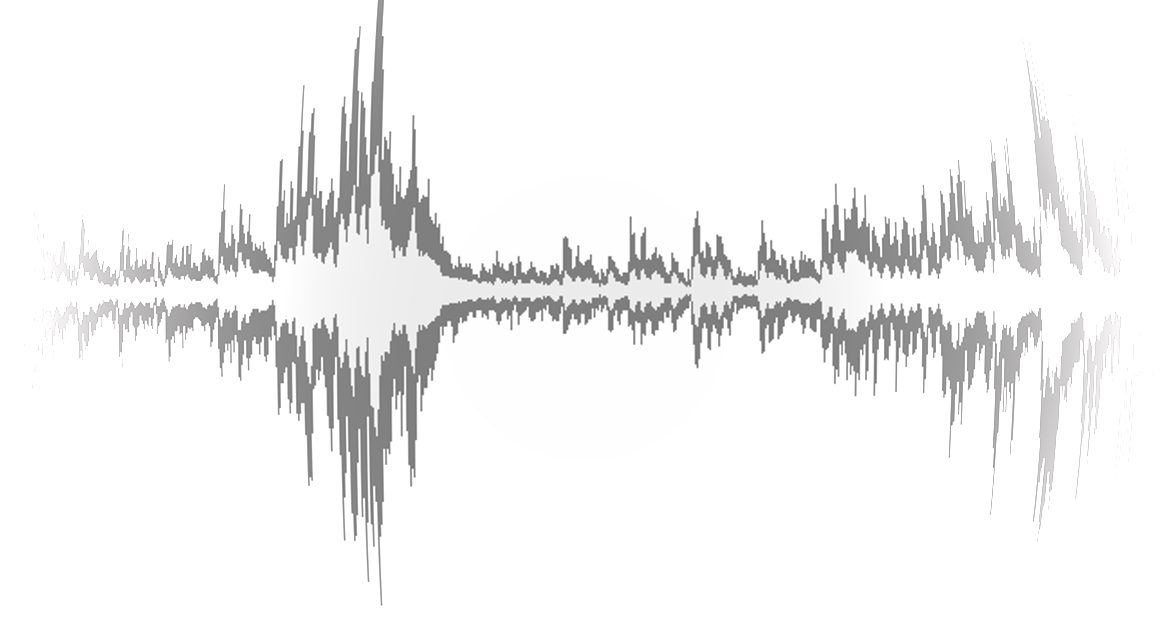
\includegraphics[width=\textwidth,height=3cm]{title}}


\begin{frame}
    \titlepage
    %\vspace{-5mm}
    \begin{flushright}
        \href{http://www.gtcmt.gatech.edu}{
\includegraphics[height=.8cm,keepaspectratio]{../shared/Logo_GTCMT_black}}
    \end{flushright}
\end{frame}


\section[intro]{introduction}
\begin{frame}{dynamics processing}{introduction}
	\begin{itemize}
		\item	\textbf{basic principle}
			\begin{itemize}
				\item	\textit{apply time-variant audio gain} 
                \item   gain depends on signal properties or external factors
			\end{itemize}
		\pause
        \bigskip
		\item	\textbf{applications}
			\begin{itemize}
				\item	avoid clipping (unknown input level)
				\item	suppress noise
				\item	adjust playback level (playlist)
				\item	decrease dynamic range (environmental noise)
				\item	increase loudness/energy (commercials)
				\item	adjust (recording) level
			\end{itemize}
	\end{itemize}
\end{frame}
\begin{frame}{dynamics processing}{introduction: effects}
	\begin{itemize}
		\item	(noise) \textbf{gate}
			\begin{itemize}
				\item	suppression of low levels in pauses
			\end{itemize}
		\pause
        \smallskip
		\item	\textbf{compressor}
			\begin{itemize}
				\item	reduction of the dynamic range
			\end{itemize}
		\pause
        \smallskip
		\item	\textbf{expander}
			\begin{itemize}
				\item	expansion of the dynamic range
			\end{itemize}
		\pause
        \smallskip
		\item	\textbf{limiter}
			\begin{itemize}
				\item	limitation of maximum gain
			\end{itemize}
		\pause
        \smallskip
		\item	\textbf{AGC} (automatic gain control)
			\begin{itemize}
				\item	slow adaptation of recording/payback gain
			\end{itemize}
	\end{itemize}
\end{frame}

\begin{frame}{dynamics processing}{overview}
    \begin{figure}
		\begin{center}
        \begin{picture}(50,25)

            %boxes
            \put(13,0){\framebox(10,10){\tiny{\shortstack[c]{Level\\ Detect.}}}}
            \put(28,0){\framebox(10,10){\tiny{\shortstack[c]{Gain\\ Comp.}}}}

		
            %lines horizontal
            \put(0,20){\vector(1,0){39}}
            \put(41,20){\vector(1,0){10}}

            \put(10,5){\vector(1,0){3}}
            \put(38,5){\line(1,0){2}}
            \put(23,5){\vector(1,0){5}}
            
            %lines vertical
            \put(10,20){\line(0,-1){15}}
            
            \put(40,5){\vector(0,1){14}}
            
            %circles
            \put(38.5,19){$\otimes$} %40,20
            
            \put(10,20){\circle*{1}}

            %text
            \put(0,21){\footnotesize{\shortstack[c]{$x(i)$}}}
            \put(48,21){\footnotesize{\shortstack[c]{$y(i)$}}}
            \put(42,17){\footnotesize{\shortstack[c]{$g(i)$}}}

        \end{picture}
		\end{center}
    \end{figure}
	\begin{equation*}
		y(i) = x(i) \cdot g\textcolor{gtgold}{(i)}
	\end{equation*}	
	\pause
	
	computation of $g(i)$ usually depends on
	\begin{enumerate}
		\item	input signal \textit{level}
		\item	properties \& characteristics of the dynamics processor
		\item	time-based control mechanism
	\end{enumerate}
\end{frame}

\section{level detection}
\begin{frame}{dynamics processing}{level detection}
	\vspace{-3mm}
    \begin{itemize}
        \item typical measures
    \begin{itemize}
		\item	\textbf{peak}:\\ physical measure of maximum amplitude
		\item	\textbf{rms}:\\ physical measure of power level
		\item	\textbf{loudness model}:\\ models of loudness perception (dBA, Zwicker, BS.1770)
		\vspace{5mm}
    \end{itemize}
    \pause
    \item   \textbf{level computation}

		\begin{equation*}
			v_\mathrm{dB}(i) = 20\cdot\log_{10}\left(\frac{v(i)}{v_0}\right)
		\end{equation*}
	
		\pause
		\begin{itemize}
			\item	$v_0$: reference constant (\unit[0]{dB} point)
			
					digital: $v_0 = 1$ $\Rightarrow \unit{dBFS}$
			\item	scaling	factor: \unit[1]{dB} $\approx$ JNDL
		\end{itemize}

	\end{itemize}
\end{frame}
%\begin{frame}{dynamics processing}{level detection: human intensity perception}
	%decibel scale is \textit{not} loudness scale:
	%\begin{itemize}
		%\item	equal-sized steps on the decibel scale not perceived as equal-sized loudness steps
	%\end{itemize}
	%
	%\pause
	%\bigskip
	%perceptual loudness depends on
	%\begin{itemize}
		%\item	frequency
		%\item	cochlear resolution
		%\item	masking effects
	%\end{itemize}
	%\vspace{-20mm}
	%\begin{figure}
		%\flushright
			%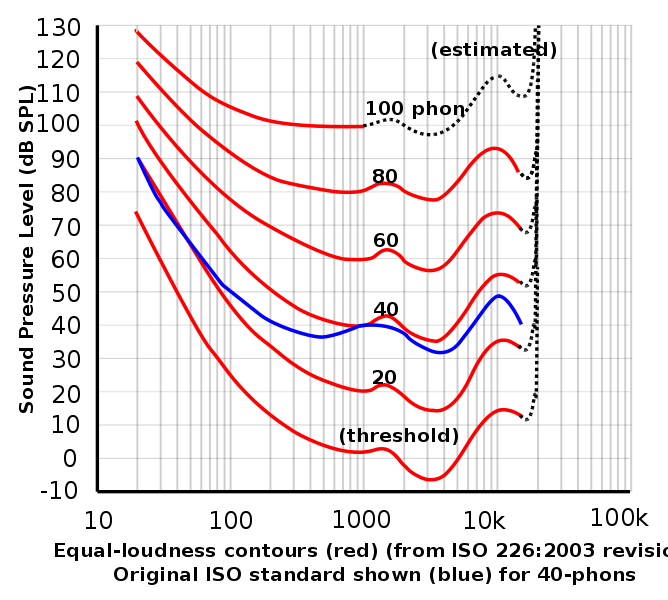
\includegraphics[scale=.25]{graph/equalloudness}
	%\end{figure}
%\end{frame}
\begin{frame}{dynamics processing}{level detection: root mean square 1/2}
	\begin{equation*}\label{eq:rms}
		v_{\mathrm{RMS}}(n) = \sqrt{\frac{1}{\mathcal{K}}\sum\limits_{i=i_{\mathrm{s}}(n)}^{i_{\mathrm{e}}(n)}{x(i)^2}}
	\end{equation*}
	\begin{figure}
		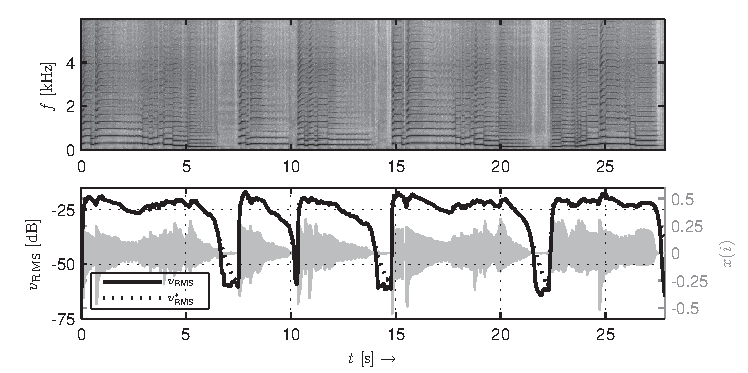
\includegraphics[scale=.7]{rms}
	\end{figure}
\end{frame}
\begin{frame}{dynamics processing}{level detection: root mean square 2/2}
			%\begin{itemize}
				%\item	measure of power
				%\item	integration time:
				%\begin{footnotesize}
					%\begin{equation*}
						%T_\mathrm{I} = \frac{i_\mathrm{e}(n)-i_\mathrm{s}(n)}{f_\mathrm{s}}
					%\end{equation*}
				%\end{footnotesize}
			%\end{itemize}
			%
			%\pause
			\textbf{sample-by-sample processing}:
			\begin{itemize}
				\item	reduce computational complexity
					\begin{footnotesize}
					\begin{eqnarray*}
						v^2_{\mathrm{RMS}}(n) &=& \frac{x(i_{\mathrm{e}}(n))^2 - x(i_{\mathrm{s}}(n-1))^2}{i_{\mathrm{e}}(n)-i_{\mathrm{s}}(n) + 1} + v^2_{\mathrm{RMS}}(n-1) \\
						v_{\mathrm{RMS}}(n)	&=& \sqrt{v^2_{\mathrm{RMS}}(n)}
					\end{eqnarray*}
					\end{footnotesize}
				\pause
				\item	single pole approximation
					\begin{footnotesize}
					\begin{eqnarray*}
						v_\mathrm{tmp}(i)	&=& \alpha\cdot v_\mathrm{tmp}(i-1) + (1-\alpha)\cdot x(i)^2\\
						v^*_{\mathrm{RMS}}(i)		&=& \sqrt{v_\mathrm{tmp}(i)}
					\end{eqnarray*}
					\end{footnotesize}
			\end{itemize}
\end{frame}
\begin{frame}{dynamics processing}{level detection: weighted root mean square}
		\vspace{-3mm}
		\begin{figure}
			\centering
\begin{footnotesize}
	\setcounter{iXOffset}{0}
	\setcounter{iYOffset}{5}
	\setcounter{iXBlockSize}{20}
	\setcounter{iYBlockSize}{16}
	\setcounter{iDistance}{5}
	\setcounter{iYBlockSizeDiv2}{8}
    \begin{picture}(57,26)


		\addtocounter{iYOffset}{\value{iYBlockSizeDiv2}}
		\addtocounter{iYOffset}{1}
        \put(\value{iXOffset},\value{iYOffset}){\footnotesize{\shortstack[c]{$x(i)$}}}
		\addtocounter{iYOffset}{-1}
		\addtocounter{iXOffset}{2}

        \put(\value{iXOffset},\value{iYOffset}){\vector(1,0){\value{iDistance}}}
		\addtocounter{iYOffset}{-\value{iYBlockSizeDiv2}}

		\addtocounter{iXOffset}{\value{iDistance}}
        \put(\value{iXOffset},\value{iYOffset}){\framebox(\value{iXBlockSize}, \value{iYBlockSize}){\footnotesize{\shortstack[c]{$H(z)$}}}}

		\addtocounter{iXOffset}{\value{iXBlockSize}}
		\addtocounter{iYOffset}{\value{iYBlockSizeDiv2}}
        \put(\value{iXOffset},\value{iYOffset}){\vector(1,0){\value{iDistance}}}
		\addtocounter{iYOffset}{-\value{iYBlockSizeDiv2}}

		\addtocounter{iXOffset}{\value{iDistance}}
        \put(\value{iXOffset},\value{iYOffset}){\framebox(\value{iXBlockSize}, \value{iYBlockSize}){\footnotesize{\shortstack[c]{$\mathrm{RMS}$}}}}

		\addtocounter{iXOffset}{\value{iXBlockSize}}
		\addtocounter{iYOffset}{\value{iYBlockSizeDiv2}}
        \put(\value{iXOffset},\value{iYOffset}){\vector(1,0){\value{iDistance}}}

        %text
		\addtocounter{iYOffset}{1}
		\addtocounter{iXOffset}{3}
        \put(\value{iXOffset},\value{iYOffset}){\footnotesize{\shortstack[c]{$v(n)$}}}

    \end{picture}
\end{footnotesize}
	    \end{figure}
	    
		\pause
        \vspace{-10mm}
	    $H(z)$:
	    \begin{itemize}
	    	\item	A, B, C weighting
	    	\item	RLB (BS.1770)
	    	\item	\ldots
	    \end{itemize}
	    
		\uncover<2->{
        \begin{figure}
			\centering
			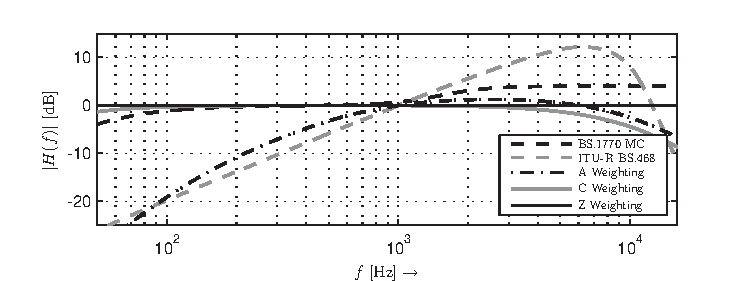
\includegraphics[scale=.7]{loudnessweighting}
			\label{fig:loudnessweighting}
		\end{figure}
        }
\end{frame}
\begin{frame}{dynamics processing}{level detection: peak detection (PPM) 1/2}
		\begin{figure}
			\centering
				\begin{footnotesize}
					\begin{picture}(100,40)(0,0)
			
						\put(-0.5,30){\circle{1}}
						\put(0,30){\vector(1,0){10}}
				
						\put(10,25){\framebox(10,10){}}
							\put(11,30){\line(1,0){8}}
							\put(15,26){\line(0,1){8}}
							\put(15,30){\line(1,1){4}}
							\put(15,30){\line(-1,1){4}}
									
						\put(20,30){\vector(1,0){5.4}}
			
						\put(25.2,28.5){\LARGE{$\oplus$}}
						
						\put(29.6,30){\vector(1,0){5.4}}
							
						\put(35,25){\framebox(10,10){}}
							\put(36,30){\line(1,0){8}}
							\put(40,26){\line(0,1){8}}
							\put(40,30){\line(1,1){4}}
						
						\put(45,30){\vector(1,0){5.4}}
			
						\put(50.2,28.5){\LARGE{$\otimes$}}
						
						\put(54.6,30){\vector(1,0){5.8}}
			
						\put(60.2,28.5){\LARGE{$\oplus$}}
						
						\put(64.6,30){\vector(1,0){5.8}}
			
						\put(70.2,28.5){\LARGE{$\oplus$}}
						
						\put(74.6,30){\vector(1,0){25.4}}
			
			
						\put(95,10){\vector(-1,0){5}}
							
						\put(80,5){\framebox(10,10){$z^{-1}$}}
			
						\put(80,10){\line(-1,0){52.5}}
			
			
			
						\put(95,30){\circle*{1}}
						\put(95,30){\line(0,-1){20}}
			
						\put(27.5,10){\vector(0,1){17.9}}
			
						\put(62.5,10){\circle*{1}}
						\put(62.5,10){\vector(0,1){17.9}}
			
						\put(72.5,10){\circle*{1}}
						\put(72.5,10){\vector(0,1){7.9}}
			
						\put(70.2,18.5){\LARGE{$\otimes$}}
			
						\put(72.5,22.1){\vector(0,1){5.8}}
						
						
						\put(0,34){\shortstack[c]{$x(i)$}}
						
						\put(21,34){\shortstack[c]{$|x(i)|$}}
						
						\put(29,26){\shortstack[c]{$-$}}
						
						\put(52,32.5){\shortstack[c]{$\alpha_\mathrm{AT}$}}
						
						\put(75,19){\shortstack[c]{$\lambda$}}
			
						\put(74,26){\shortstack[c]{$-$}}
						
						
						\put(95,34){\shortstack[c]{$v_{\mathrm{PPM}}(i)$}}
					\end{picture}
				\end{footnotesize}
		\end{figure}	
		\begin{itemize}
			\only<1>{
			\item[]
			\item[]
			\item[]
			\item[]
			}
			\only<2-3>{
			\item \textbf{release state} ($|x(i)| \leq v_{\mathrm{PPM}}(i-1)\Rightarrow\lambda = \alpha_\mathrm{RT}$)
				\invisible<2>{
				\begin{eqnarray*}
					v_{\mathrm{PPM}}(i) &=& v_{\mathrm{PPM}}(i-1) - \alpha_\mathrm{RT}\cdot v_{\mathrm{PPM}}(i-1)\nonumber\\
					\pause
								&=& (1-\alpha_\mathrm{RT})\cdot v_{\mathrm{PPM}}(i-1) 
				\end{eqnarray*}
				}
			}
			\only<4-5>{
			\item \textbf{attack state} ($|x(i)| > v_{\mathrm{PPM}}(i-1)\Rightarrow\lambda = 0$)
				\invisible<4>{
				\begin{eqnarray*}
					v_{\mathrm{PPM}}(i) &=& \alpha_\mathrm{AT}\cdot\big(|x(i)| - v_{\mathrm{PPM}}(i-1)\big) + v_{\mathrm{PPM}}(i-1)\nonumber\\
					\pause
								&=& \alpha_\mathrm{AT}\cdot |x(i)| + (1-\alpha_\mathrm{AT})\cdot v_{\mathrm{PPM}}(i-1) 
				\end{eqnarray*}
				}
			}
		\end{itemize}
\end{frame}
\begin{frame}{dynamics processing}{level detection: peak detection (PPM) 2/2}
		\begin{figure}
			\centering
				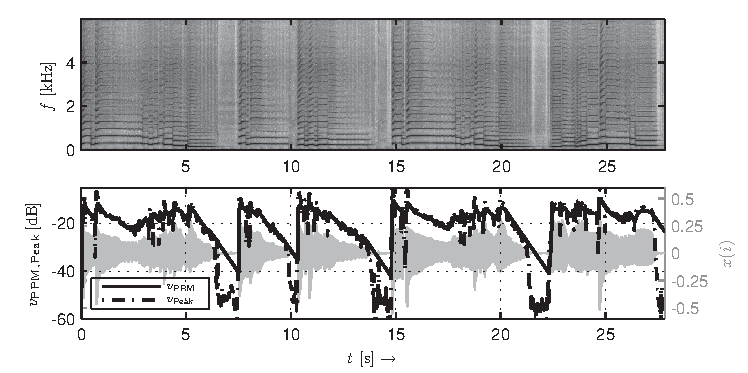
\includegraphics[scale=.7]{ppm}
			\label{fig:ppm_level}
		\end{figure}
\end{frame}	

\section{response curve}
\begin{frame}{dynamics processing}{response curve: limiter}
	\only<1>{
	\begin{figure}
		\centering
			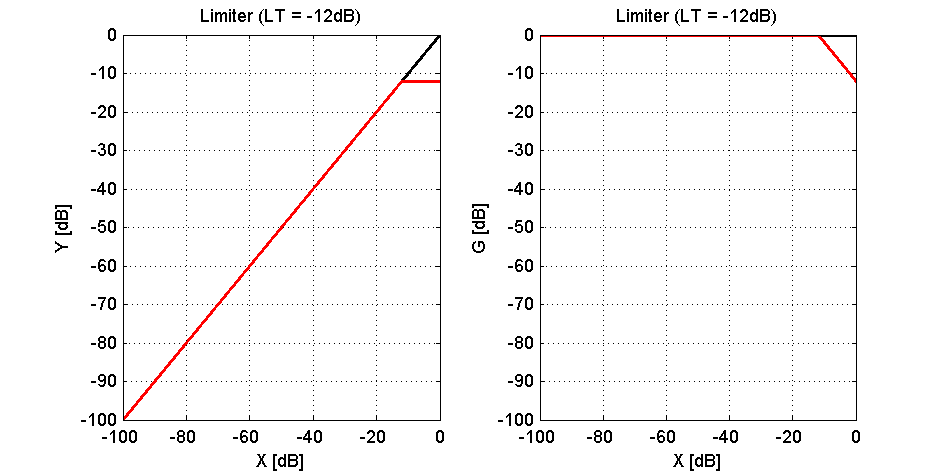
\includegraphics[scale=.6]{graph/fx3_lmt-01}
	\end{figure}
	}
	\only<2>{
		\begin{figure}
			\centering
				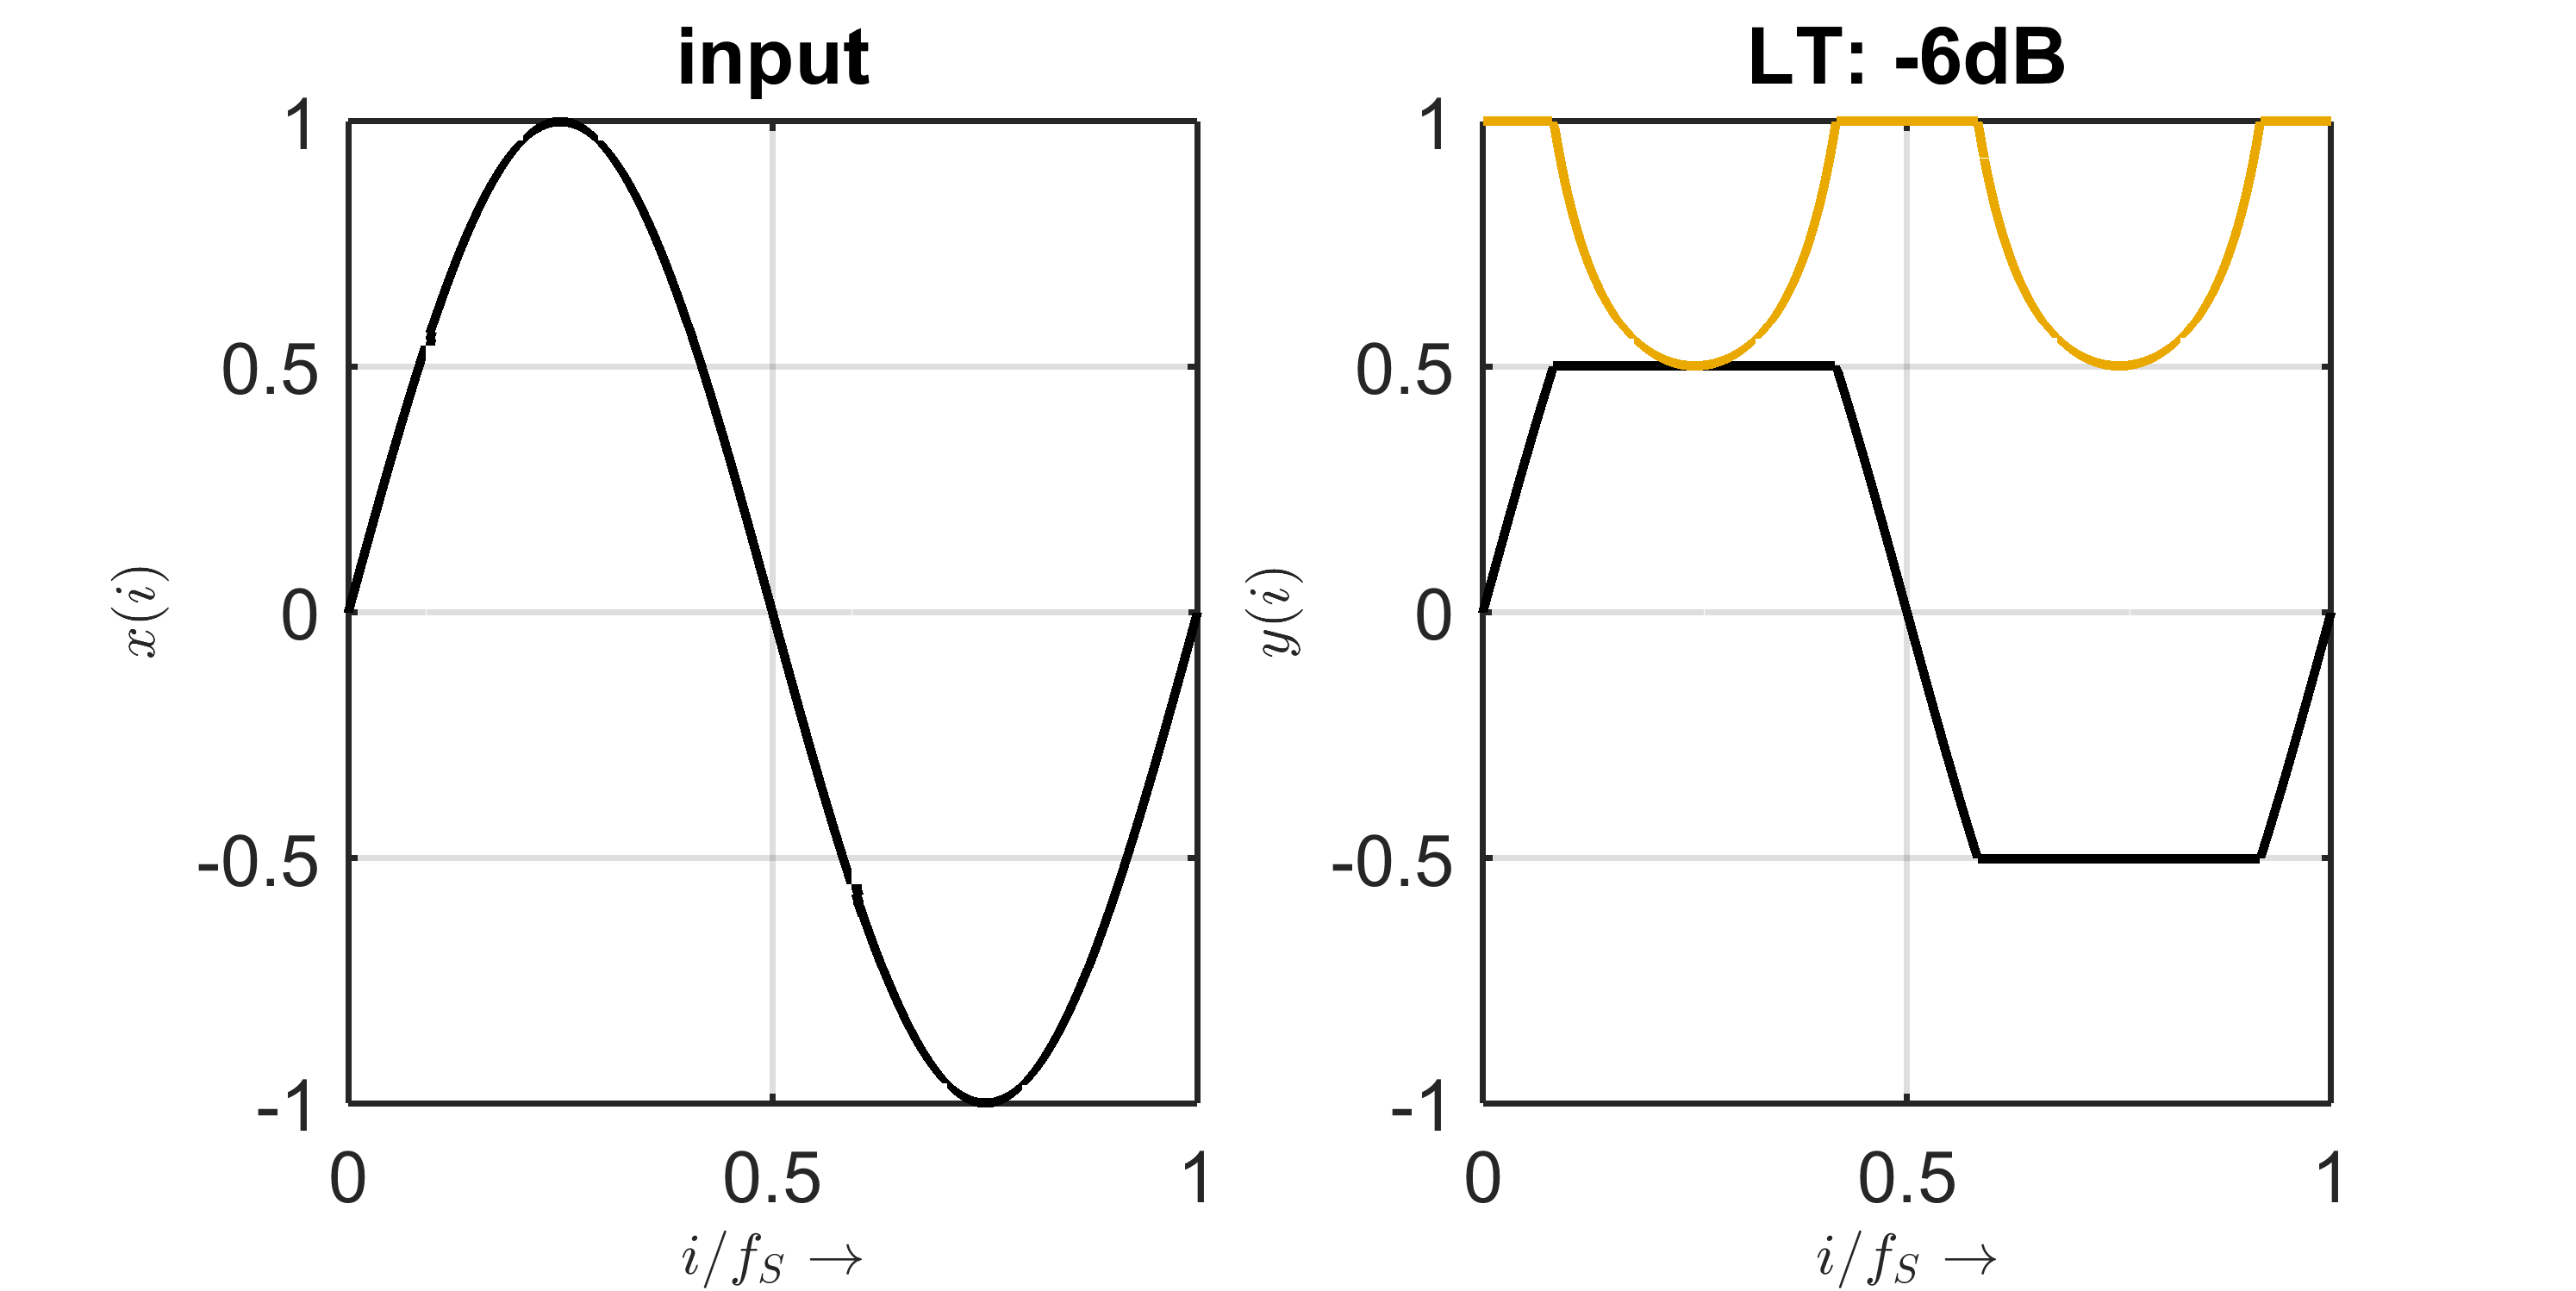
\includegraphics[scale=.7]{graph/dynamicsresponsecurve_1}
		\end{figure}

		param $LT=\unit[-9]{dB}$ \includeaudio{svdynamicsresponsecurve_1}
	}
\end{frame}
\begin{frame}{dynamics processing}{response curve: compressor}
	\only<1>{
	\begin{figure}
		\centering
			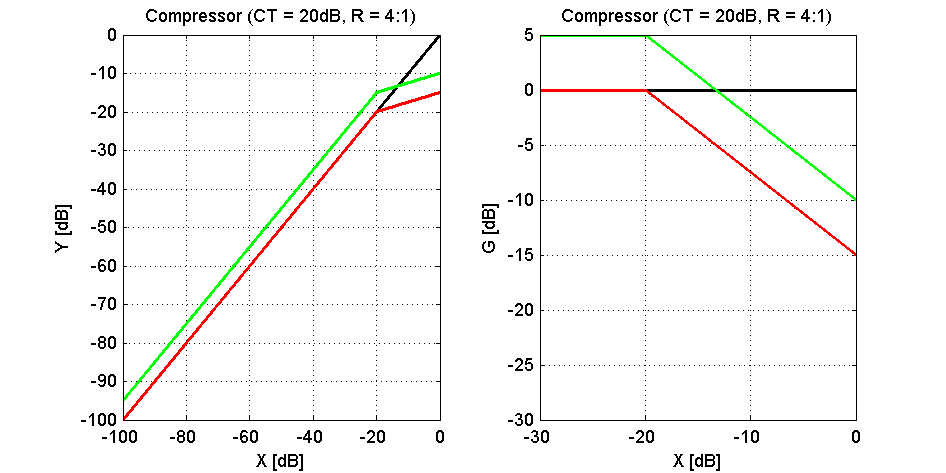
\includegraphics[scale=.6]{graph/fx3_comp-01}
	\end{figure}
	}
	\only<2>{
		\begin{figure}
			\centering
				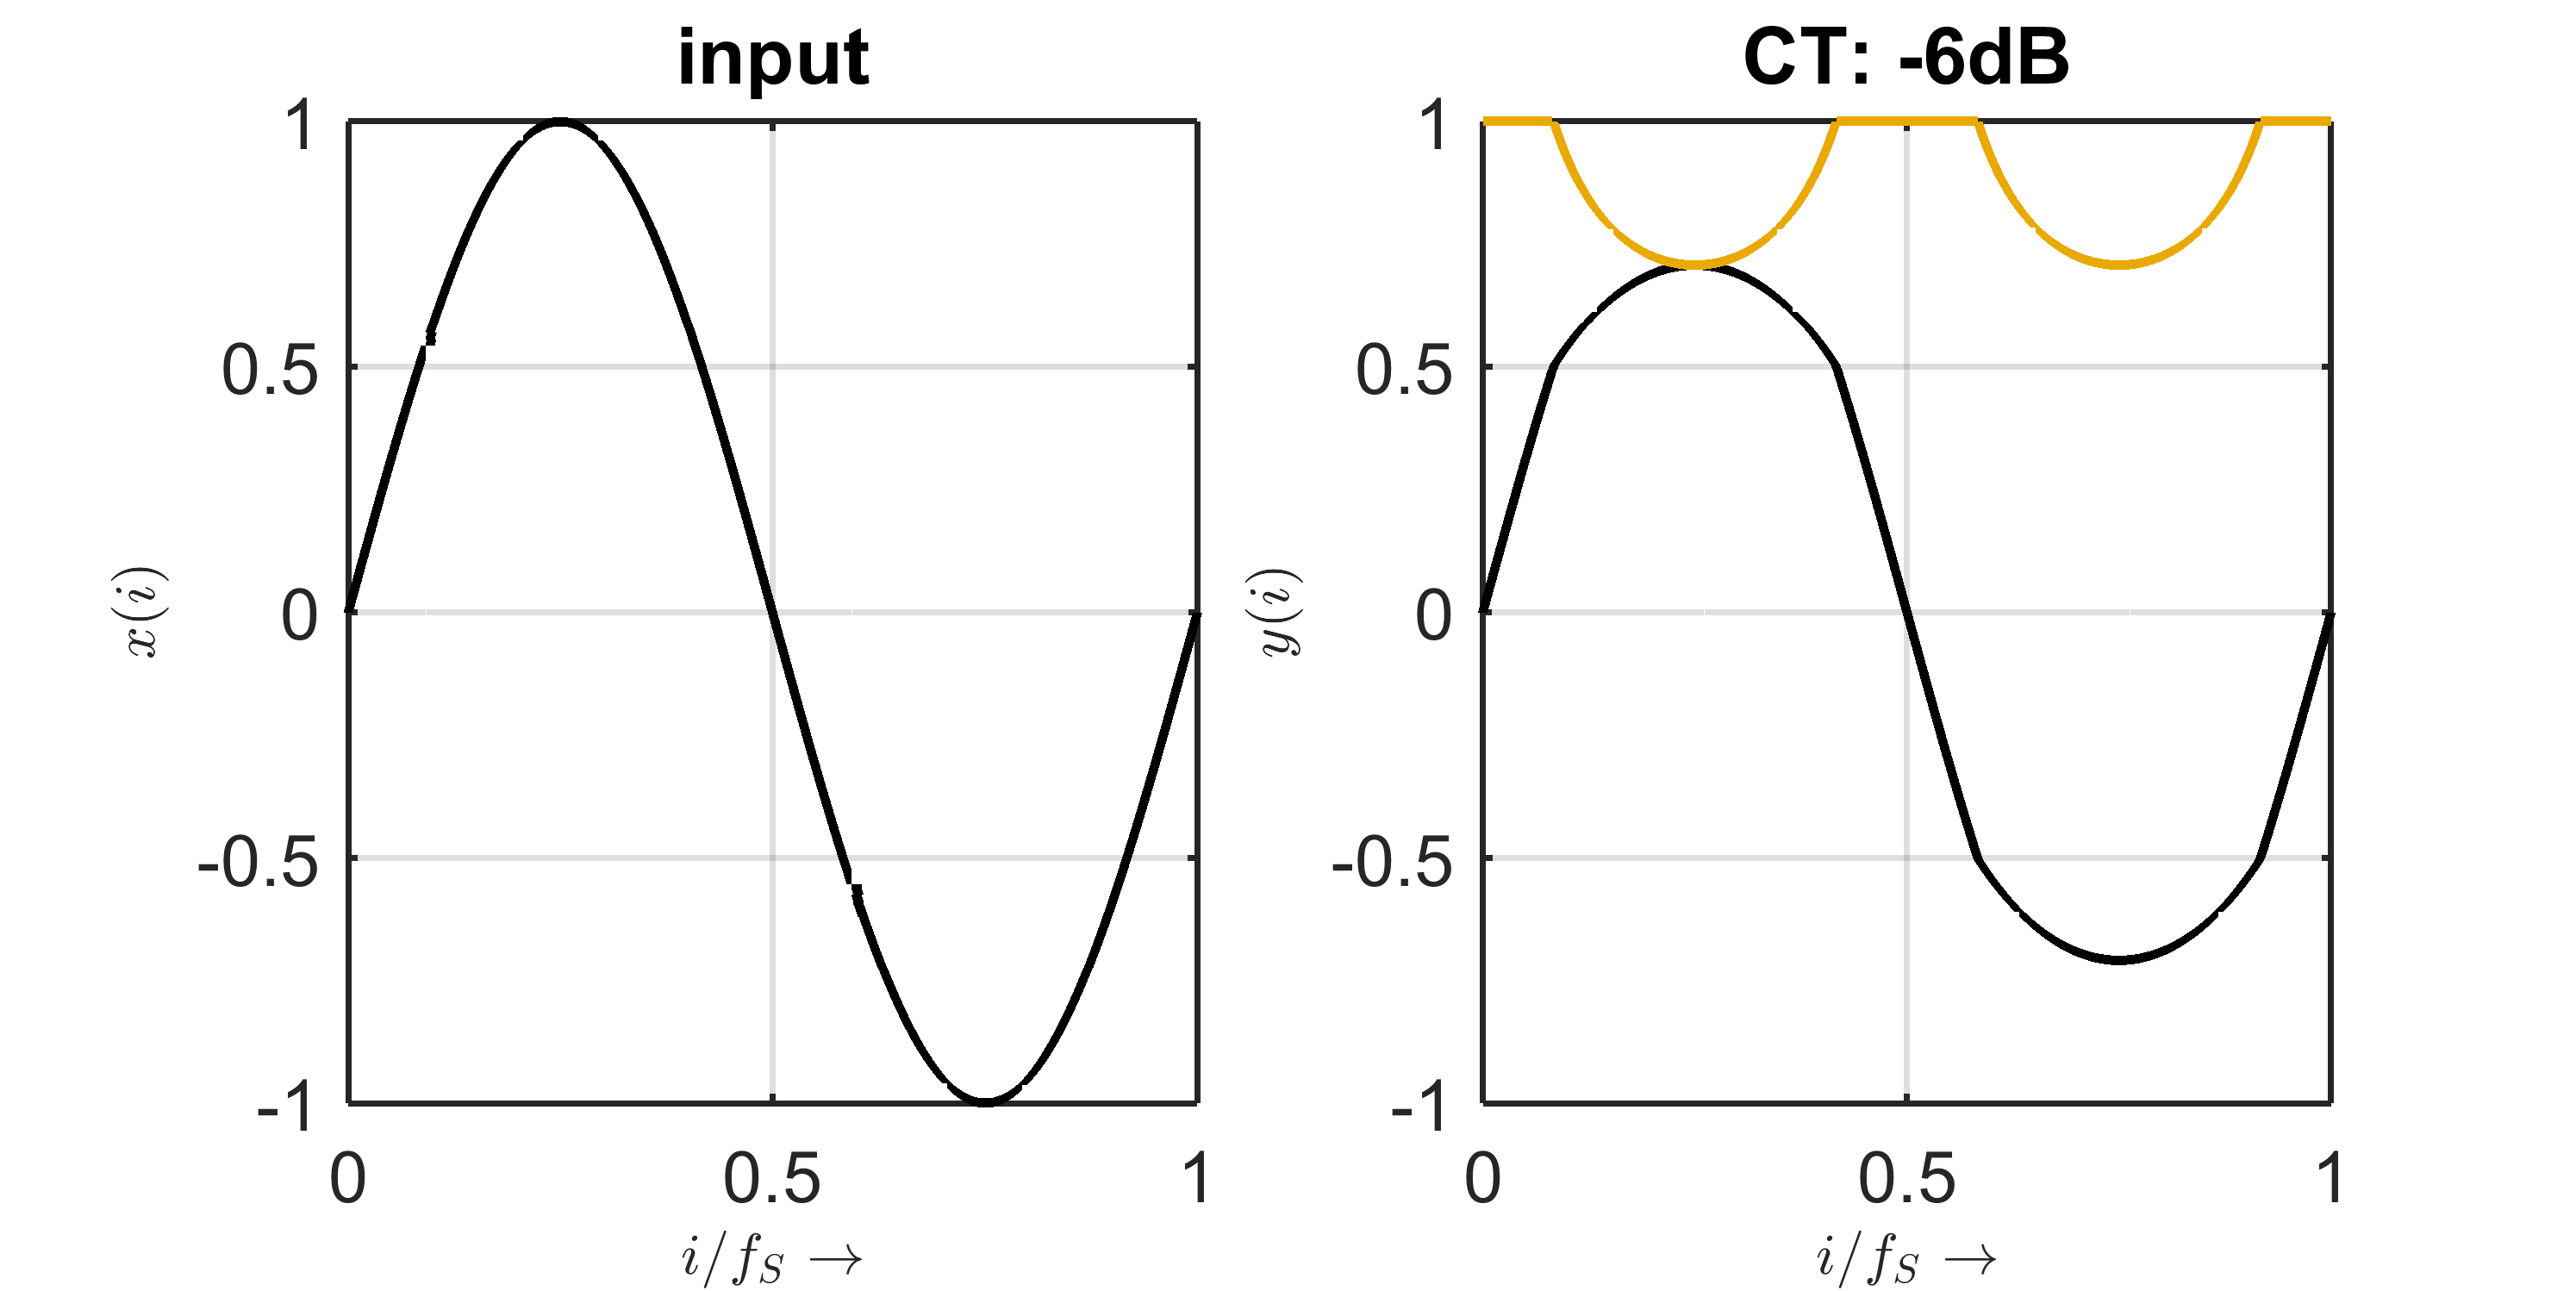
\includegraphics[scale=.7]{graph/dynamicsresponsecurve_2}
		\end{figure}

		param $CT=\unit[-9]{dB}$\includeaudio{svdynamicsresponsecurve_2}
	}
\end{frame}
\begin{frame}{dynamics processing}{response curve: expander}
	\only<1>{
	\begin{figure}
		\centering
			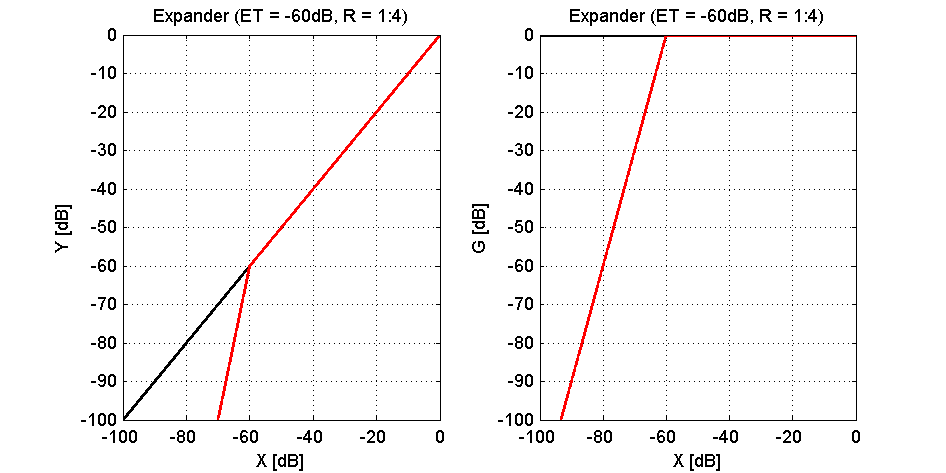
\includegraphics[scale=.6]{graph/fx3_exp-01}
	\end{figure}
	}
	\only<2>{
		\begin{figure}
			\centering
				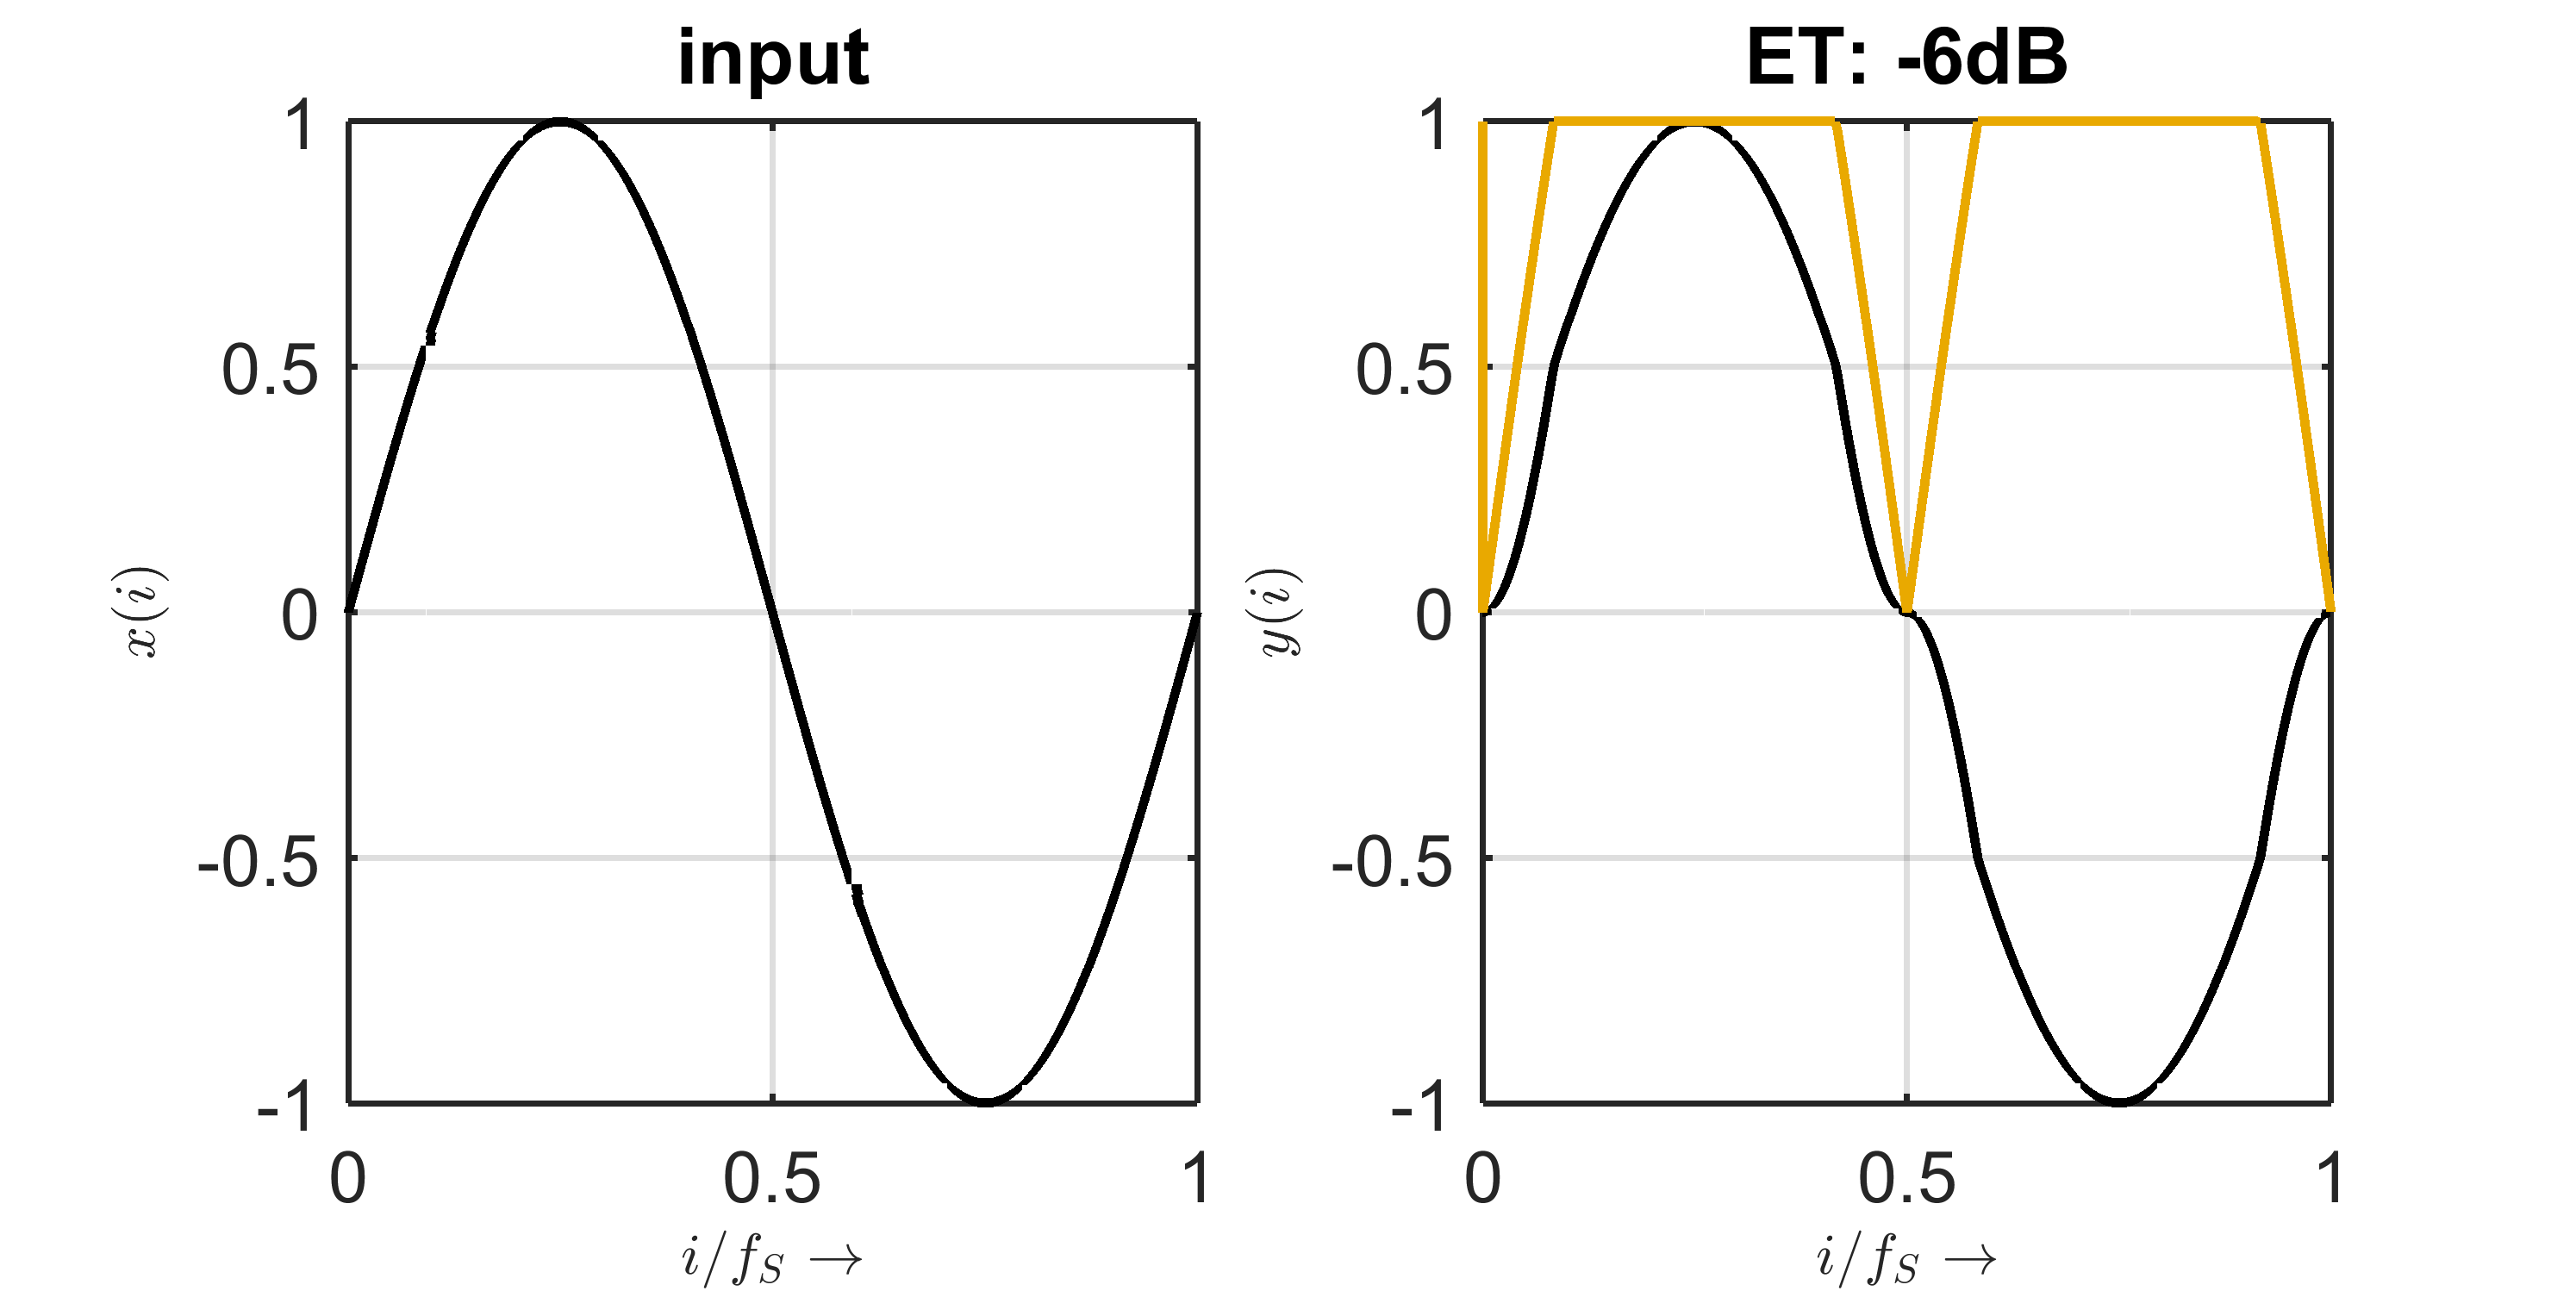
\includegraphics[scale=.7]{graph/dynamicsresponsecurve_3}
		\end{figure}

		param $ET=\unit[-6]{dB}$\includeaudio{svdynamicsresponsecurve_3}
	}
\end{frame}
\begin{frame}{dynamics processing}{response curve: noise gate}
	\only<1>{
	\begin{figure}
		\centering
			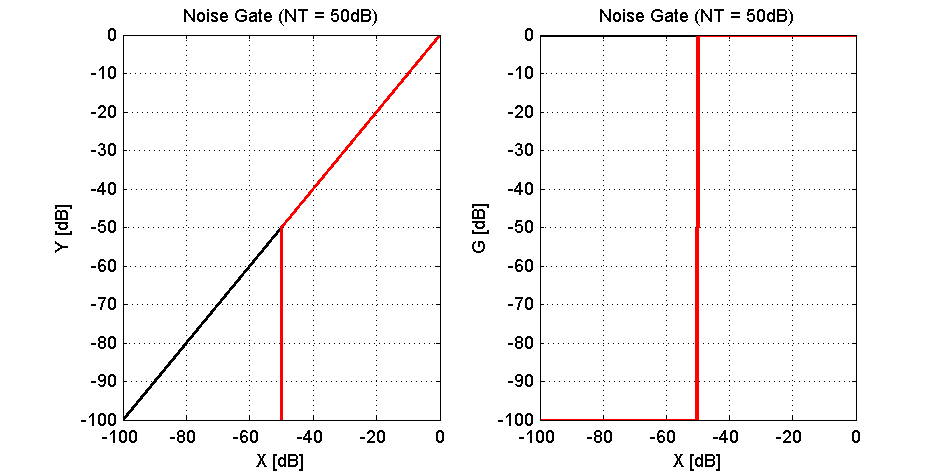
\includegraphics[scale=.6]{graph/fx3_gate-01}
	\end{figure}
	}
	\only<2>{
		\begin{figure}
			\centering
				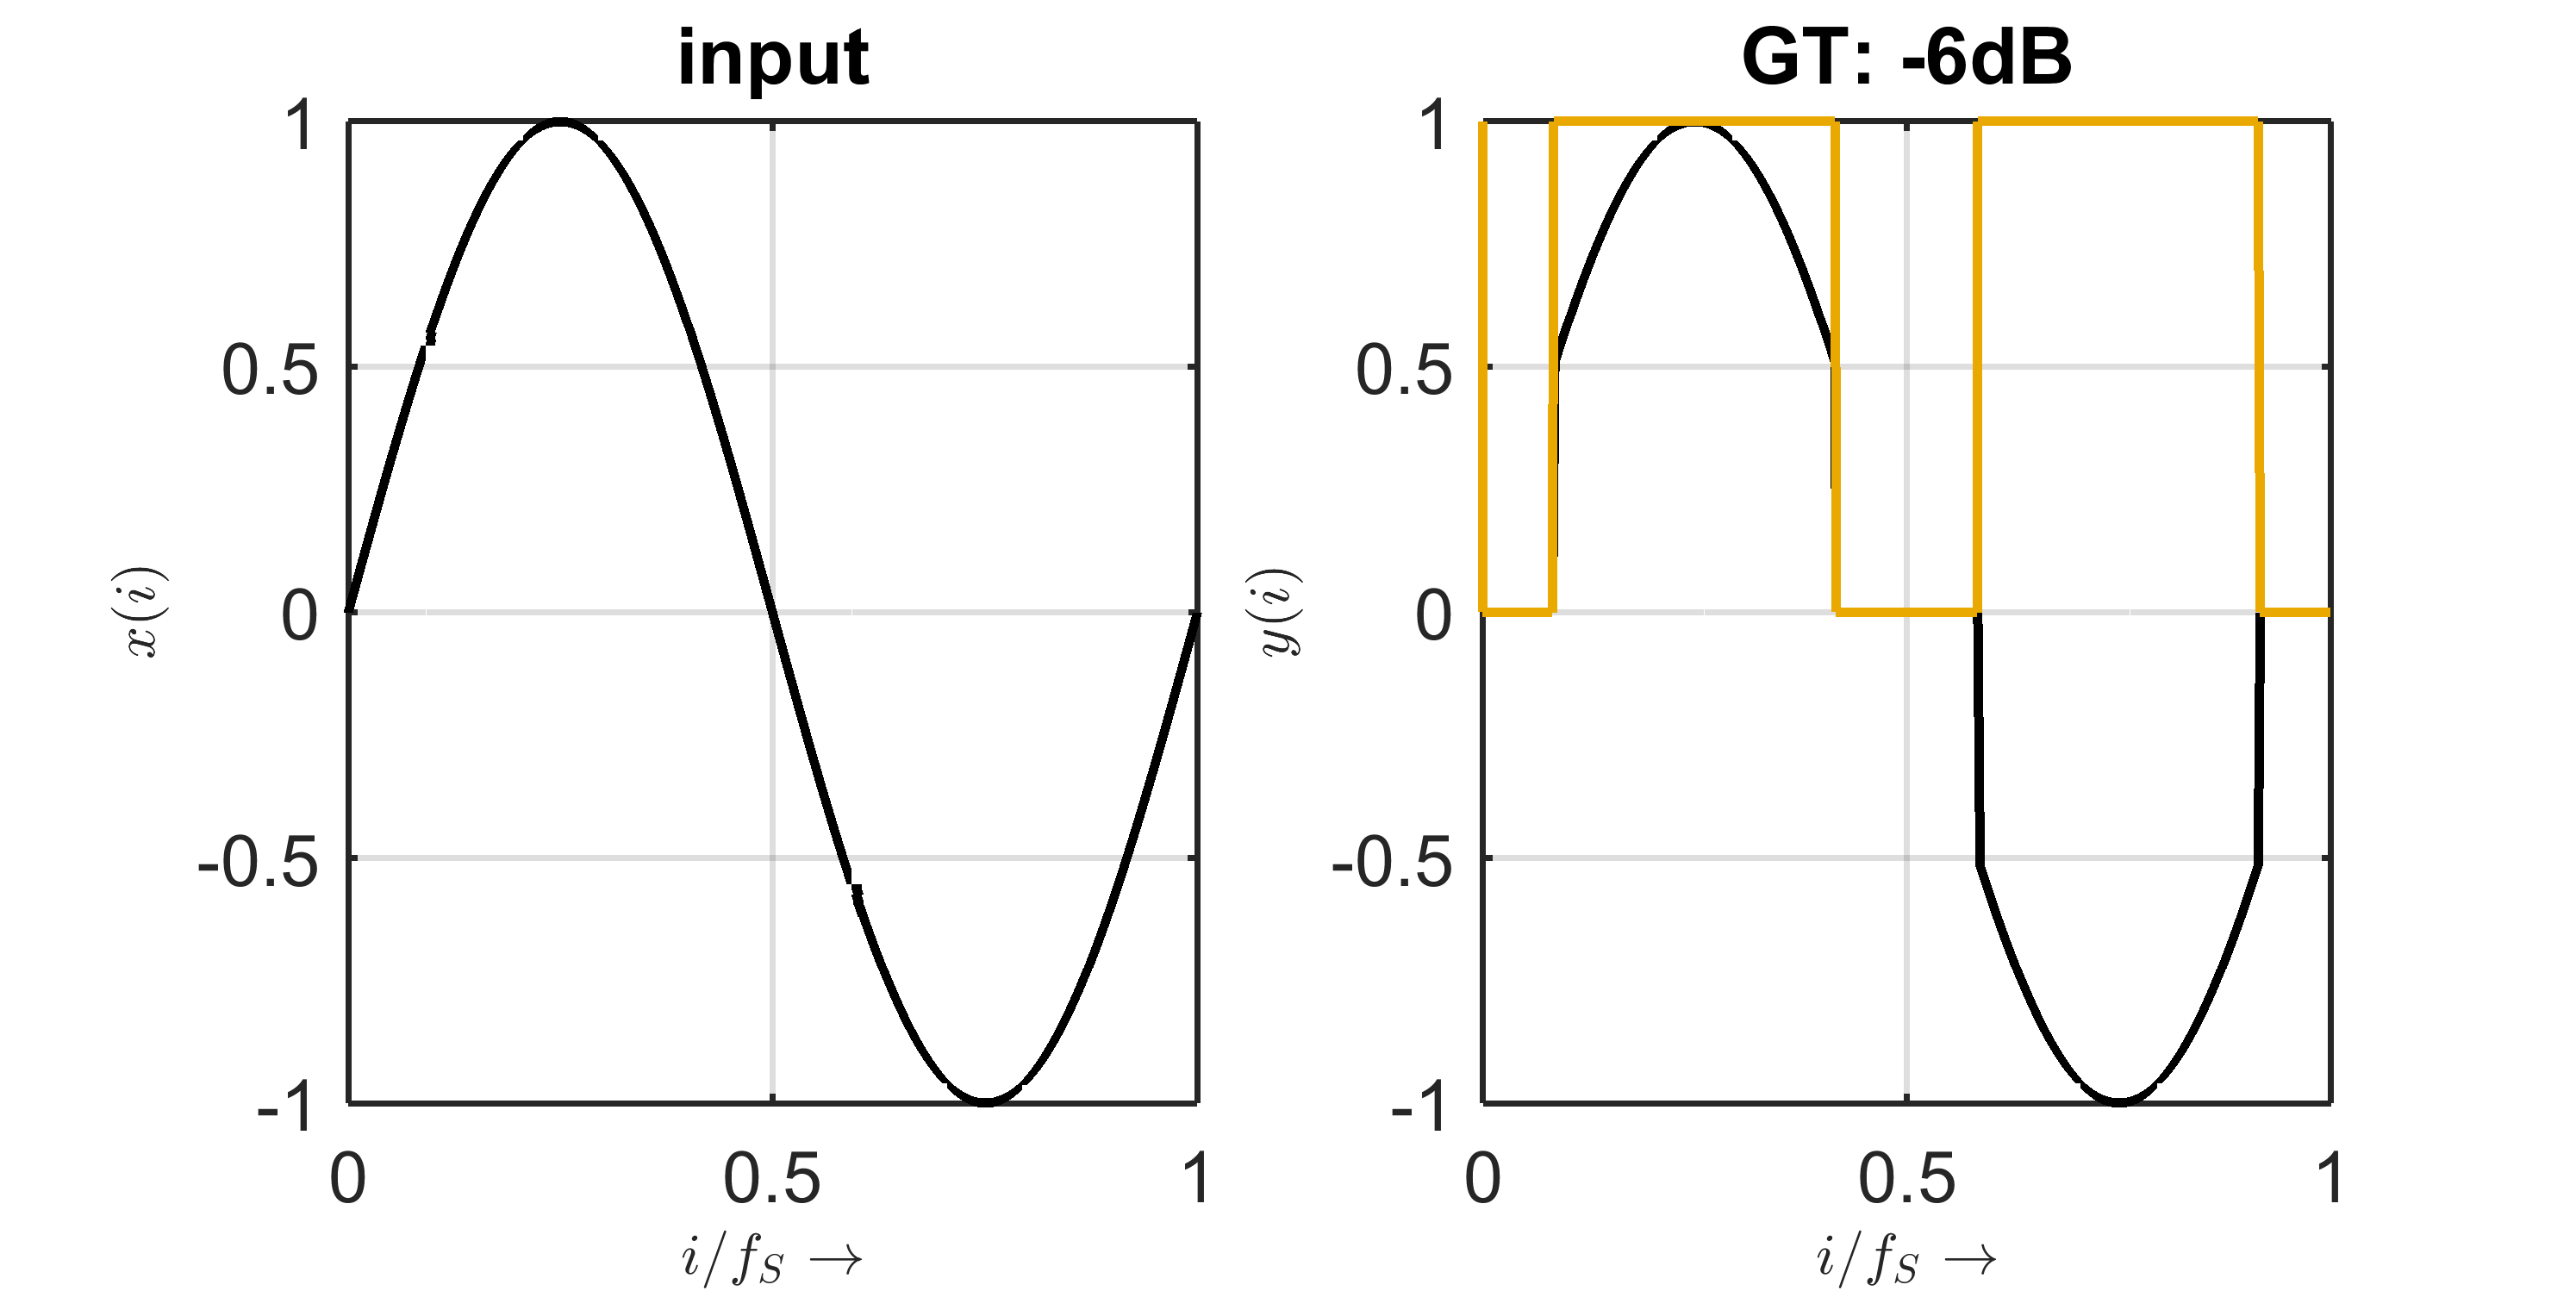
\includegraphics[scale=.7]{graph/dynamicsresponsecurve_4}
		\end{figure}

		param $NT=\unit[-12]{dB}$\includeaudio{svdynamicsresponsecurve_4}
	}
\end{frame}

\begin{frame}{dynamics processing}{response curve: mathematical description (compressor)}
	\vspace{-2mm}
    logarithmic description, nonlinear part
    \bigskip
	\begin{itemize}
		\item	 \textbf{output}:
			$Y = g(X) + X\quad [\unit{dB}]$
		\pause
		\item	\textbf{ratio}:
			$R = \frac{\Delta L_i}{\Delta L_o}$
		\pause
		\item	\textbf{slope}:
			$CS = 1-\frac{1}{R}$
		\pause
		\item	\textbf{linear equation} (offset CT):
			$Y = \frac{1}{R}\left(X-CT\right) + CT$
		\pause
		\item	\textbf{gain} ($g = Y-X$):
			\begin{footnotesize}\begin{eqnarray*}
				g &=& \frac{1}{R}(X-CT) + CT - X\\
				\pause
				  &=& \left(1-\frac{1}{R}\right)\cdot (CT-X)\\
                  &=& CS\cdot(CT-X)
			\end{eqnarray*}\end{footnotesize}
	\end{itemize}
\end{frame}
\begin{frame}{dynamics processing}{response curve: mathematical description (summary 1/2)}
	\vspace{-2mm}
    logarithmic description, nonlinear part
    \bigskip
	\begin{itemize}
		\item	\textbf{limiter}
			\begin{footnotesize}\begin{eqnarray*}
				R &=& \infty\\
				Y &=& LT\\
				g &=& LT-X
			\end{eqnarray*}\end{footnotesize}
		\pause
		\item	\textbf{compressor}
			\begin{footnotesize}\begin{eqnarray*}
				R &>& 1\\
				Y &=& \frac{1}{R}\left(X-CT\right) + CT\\
				g &=& \left(1-\frac{1}{R}\right)\cdot (CT-X)
			\end{eqnarray*}\end{footnotesize}
	\end{itemize}
\end{frame}
\begin{frame}{dynamics processing}{response curve: mathematical description (summary 2/2)}
	\vspace{-2mm}
    logarithmic description, nonlinear part
    \bigskip
	\begin{itemize}
		\item	\textbf{expander}
			\begin{footnotesize}\begin{eqnarray*}
				R &<& 1\\
				Y &=& \frac{1}{R}\left(X-ET\right) + ET\\
				g &=& \left(1-\frac{1}{R}\right)\cdot (ET-X)
			\end{eqnarray*}\end{footnotesize}
		\pause
		\item	\textbf{gate}
			\begin{footnotesize}\begin{eqnarray*}
				R &=& 0\\
				Y &=& -\infty\\
				g &=& -\infty
			\end{eqnarray*}\end{footnotesize}
	\end{itemize}
\end{frame}

\section{smoothing}
\begin{frame}{dynamics processing}{smoothing: attack and release 1/2}
	\begin{figure}
		\centering
			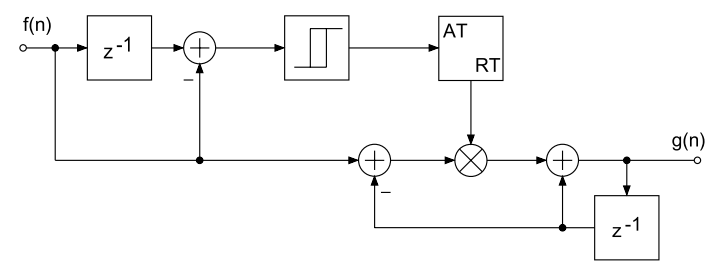
\includegraphics[scale=.5]{graph/smooth_control}
	\end{figure}
	\begin{itemize}
		\item	$\alpha_{AT}$: attack constant
		\item	$\alpha_{RT}$: release constant
	\end{itemize}
	
	\pause
	\begin{eqnarray*}
		g(n) &=& \alpha\cdot(f(n)-g(n-1)) + g(n-1)\nonumber\\
		\pause
			&=& \alpha f(n) + (1-\alpha)\cdot g(n-1)
	\end{eqnarray*}
\end{frame}

\begin{frame}{dynamics processing}{smoothing: attack and release 2/2}
	\vspace{-3mm}
    \begin{figure}
		\centering
			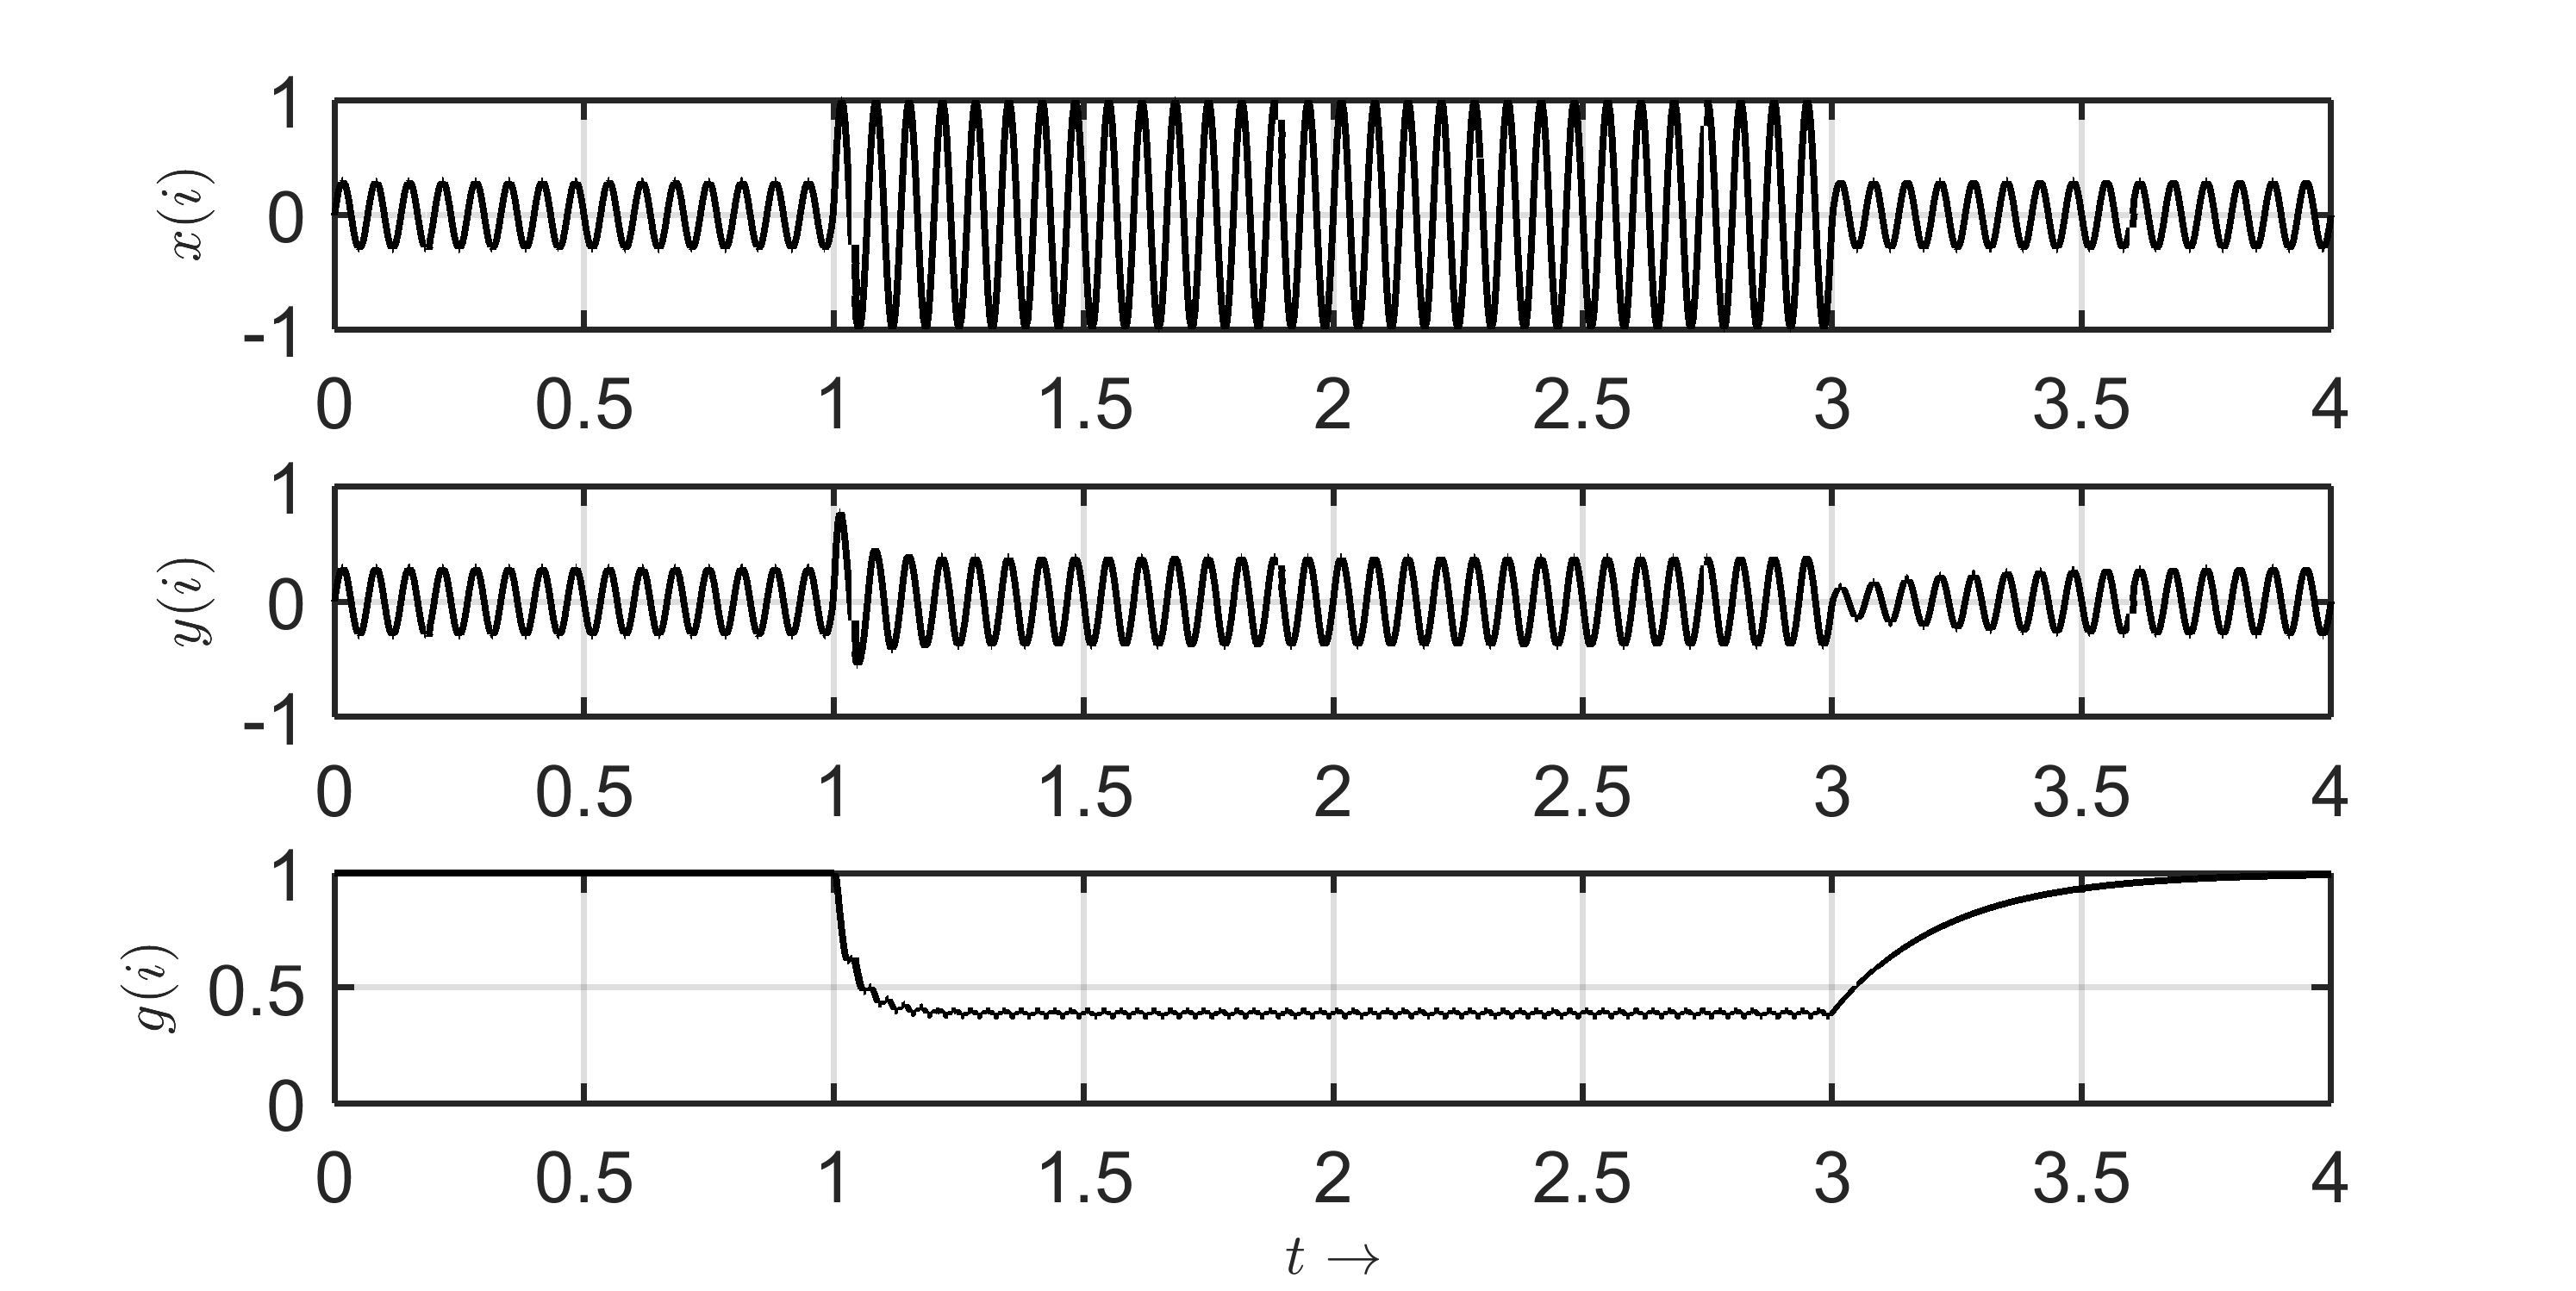
\includegraphics[scale=1]{graph/comp_sine}
	\end{figure}
\end{frame}

\begin{frame}{dynamics processing}{smoothing: attack and release coefficients}
    \begin{itemize}
        \item   single pole step response $\rightarrow g(t) = 1-e^{\frac{-t}{\tau}}$ 
        \pause
        \item   define single pole integration time between 10\% and 90\%
            \begin{eqnarray*}
                t_\mathrm{I} &=& t_{90} - t_{10}\\
                0.1 &=& 1 - e^{\frac{-t_{10}}{\tau}}\\
                0.9 &=& 1 - e^{\frac{-t_{90}}{\tau}}\\
        \pause
            \Rightarrow \nicefrac{0.9}{0.1} &=& e^{\frac{t_{90}-t_{10}}{\tau}}\\
        \pause
            \log\left(\nicefrac{0.9}{0.1}\right) &=& \nicefrac{t_{90}-t_{10}}{\tau}\\
        \pause
            t_{90}-t_{10} &=& 2.197\tau\\
            \tau &\approx& \nicefrac{t_\mathrm{I}}{2.2}
        \end{eqnarray*}

    \end{itemize}
\end{frame}

\section{overall system}
\begin{frame}{dynamics processing}{overall system: limiter}
	\begin{figure}
		\centering
			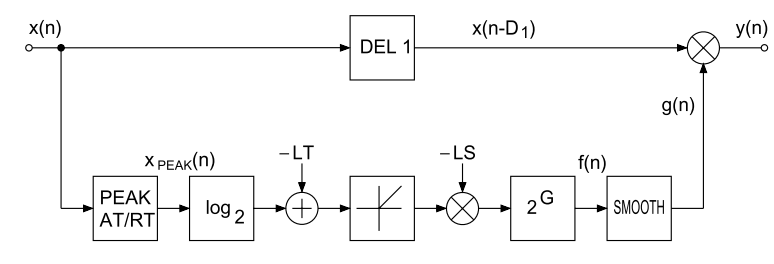
\includegraphics[scale=.5]{graph/limiter}
	\end{figure}
	\begin{equation*}
		CS = 1-\frac{1}{R} \Rightarrow LS = 1
	\end{equation*}

	\pause	
	\begin{itemize}
		\item	$X<LT\rightarrow g = 1$
		\pause
		\item	$X>LT\rightarrow g = (LT-X)$
	\end{itemize}
\end{frame}

\begin{frame}{dynamics processing}{gain visualization: combined system}
	\vspace{-3mm}\begin{figure}
		\centering
			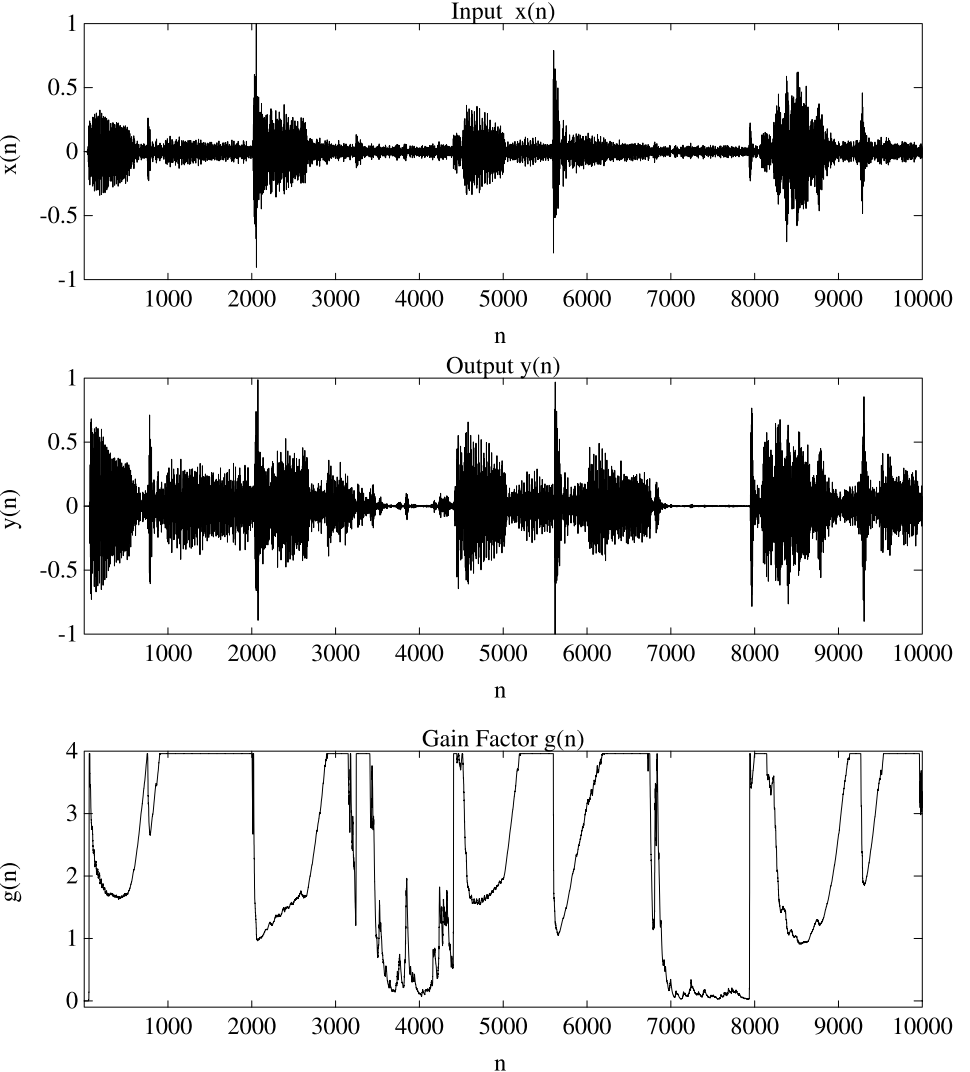
\includegraphics[scale=.25]{graph/dynamics_gain}
	\end{figure}
\end{frame}

\begin{frame}{dynamics processing}{audio examples}
    \includeaudio{sv}
    \bigskip
    \begin{itemize}
        \item Gate \includeaudio{sv_Gate}
        \item Expander \includeaudio{sv_Expander}
        \item Compressor \includeaudio{sv_Compressor}
        \item Limiter \includeaudio{sv_Limiter}
    \end{itemize}
\end{frame}

\section{variants}
\begin{frame}{dynamics processing}{variants 1/3}
	\vspace{-3mm}
    \begin{itemize}
		\item	\textbf{attack \& release constant selection}
			\begin{itemize}
				\item	depending on ``abruptness'' of change
			\end{itemize}
		\pause
        \smallskip
		\item	\textbf{hold time}
			\begin{itemize}
				\item	before release, hold gain constant (avoid pumping with low frequency signals)
			\end{itemize}
		\pause
        \smallskip
		\item	\textbf{oversampling}
			\begin{itemize}
				\item	high time resolution for peak detection
			\end{itemize}
	\end{itemize}
    \visible<3->{
    \begin{figure}[!htbp]
        \centering
            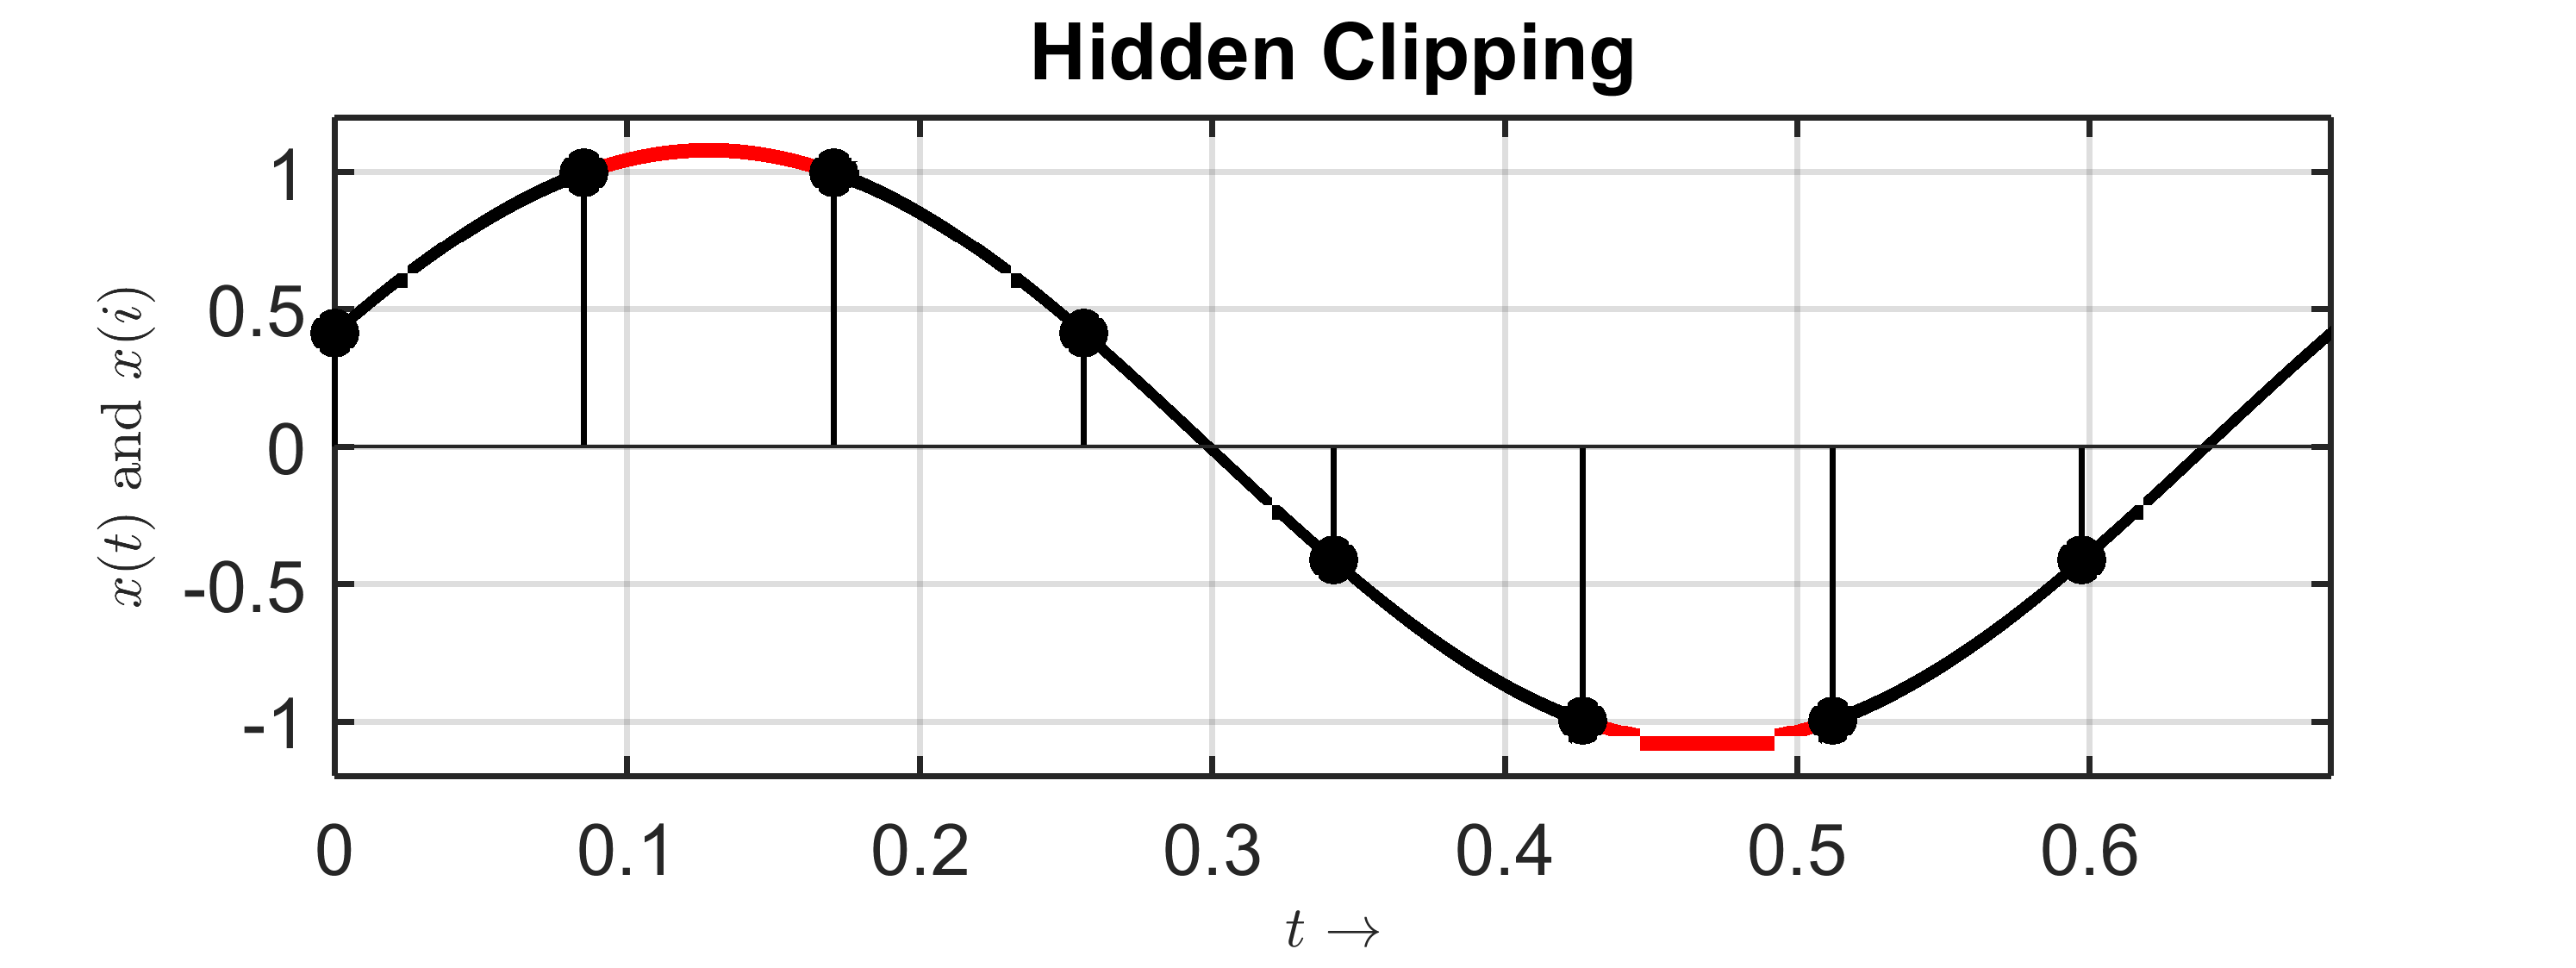
\includegraphics[scale=.6]{graph/hiddenclipping}
    \end{figure}
    }
\end{frame}

\begin{frame}{dynamics processing}{variants 2/3}
	\vspace{-3mm}
    \begin{itemize}
		\item	\textbf{stereo link}
			\begin{itemize}
				\item	consider both channels (avoid level-dependent changes of stereo image)
					\pause
					\begin{itemize}
						\item	one master channel (left or right)
						\item	mean of both channels
						\item	channel with higher level (max)
					\end{itemize}
			\end{itemize}
		\pause
        \smallskip
        \smallskip
		\item	\textbf{soft knee}
			\begin{itemize}
				\item	smooth crossover from linear area to compressed area
					\visible<4->{
                    \begin{figure}
						\flushright
							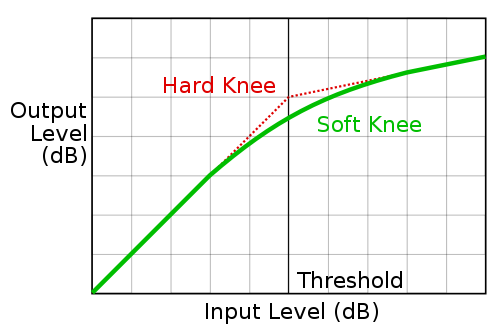
\includegraphics[scale=.2]{graph/dynamics_softknee}
					\end{figure}
                    }
					\vspace{-20mm}
					\pause
					potentially noticeable with
					\begin{itemize}
						\item	very short attack times
						\item	high compression ratios	
					\end{itemize}
			\end{itemize}
	\end{itemize}
\end{frame}

\begin{frame}{dynamics processing}{variants 3/3}
	\begin{itemize}
		\item	\textbf{side chain}
			\begin{itemize}
				\item	choose different input signal for level control (``ducking'')
			\end{itemize}
		\pause
        \bigskip
		\item	\textbf{look-ahead}
			\begin{itemize}
				\item	introduce higher delay in signal path
					\begin{itemize}
						\item	shift gain modification in time
						\item	combine ``future'' measurement with current
					\end{itemize}
			\end{itemize}
        \bigskip
		\pause
		\item	\textbf{multi-band compression}
            \begin{itemize}
                \item	apply one compressor to each frequency band
                \item	advantages:
                    \begin{itemize}
                        \item	avoid pumping: varying level in one band (e.g. bass drum) does not influence gain of other bands
                        \item	maximize power, overall loudness
                    \end{itemize}
            \end{itemize}
        
	\end{itemize}
\end{frame}

\section{params \& usage}
\begin{frame}{dynamics processing}{parameter ranges}
	\vspace{-3mm}
    \begin{itemize}
		\item	\textbf{threshold}\\
		\uncover<2->{$-120 \ldots 0$ dB}
		
		\item	\textbf{ratio}\\
		\uncover<2->{$0.05 \ldots 20$ (Limiter: $\infty$)}
		
		\item	\textbf{attack}\\
		\uncover<2->{$0 \ldots 10$ \unit{ms}}
		
		\item	\textbf{release}\\
		\uncover<2->{$20 \ldots 300$ \unit{ms}}

		\item	\textbf{hold}\\
		\uncover<2->{$0 \ldots 10$ \unit{ms}}
		
		\item	\textbf{stereo-link}\\
		\uncover<2->{On/Off}
		
		\item	\textbf{oversampling}\\
		\uncover<2->{$1 \ldots 8$}
		
		\item	\textbf{look-ahead}\\
		\uncover<2->{$0 \ldots 500$ \unit{ms}}
	\end{itemize}
\end{frame}

\begin{frame}{dynamics processing}{dynamic range target}
    \begin{figure}
        \rotatebox[origin=c]{270}{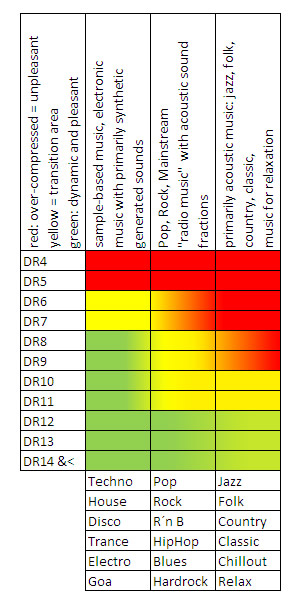
\includegraphics[scale=.5]{dynamicrange}}
    \end{figure}
\end{frame}

\section{summary}
\begin{frame}{dynamics processing}{summary}
	dynamics processing systems are
	\begin{itemize}
		\item	\textbf{time variant}:\\ gain changes over time
		\pause
		\item	\textbf{signal adaptive}:\\ gain depends on (input) signal
		\pause
		\item	sometimes \textbf{non-linear}:\\ at very short attack times (limiting)
	\end{itemize}
\end{frame}

\end{document}

